%
% Template Laporan Skripsi/Thesis 
%
% @author  Andreas Febrian, Lia Sadita 
% @version 1.03
%
% Dokumen ini dibuat berdasarkan standar IEEE dalam membuat class untuk 
% LaTeX dan konfigurasi LaTeX yang digunakan Fahrurrozi Rahman ketika 
% membuat laporan skripsi. Konfigurasi yang lama telah disesuaikan dengan 
% aturan penulisan thesis yang dikeluarkan UI pada tahun 2008.
%

%
% Tipe dokumen adalah report dengan satu kolom. 
%
\documentclass[12pt, a4paper, onecolumn, oneside, final]{report}

% Load konfigurasi LaTeX untuk tipe laporan thesis
\usepackage{uithesis}
\usepackage{graphicx}


% Load konfigurasi khusus untuk laporan yang sedang dibuat
%-----------------------------------------------------------------------------%
% Informasi Mengenai Dokumen
%-----------------------------------------------------------------------------%
% 
% Judul laporan. 
\var{\judul}{Thin-Client Pipelining dari Fast R-CNN untuk Pengenalan Batik}
% 
% Tulis kembali judul laporan, kali ini akan diubah menjadi huruf kapital
\Var{\Judul}{Thin-Client Pipelining dari Fast R-CNN untuk Pengenalan Batik}
% 
% Tulis kembali judul laporan namun dengan bahasa Ingris
\var{\judulInggris}{Thin-Client Pipelining of Fast R-CNN for Batik Recognition}

% 
% Tipe laporan, dapat berisi Skripsi, Tugas Akhir, Thesis, atau Disertasi
\var{\type}{Thesis}
% 
% Tulis kembali tipe laporan, kali ini akan diubah menjadi huruf kapital
\Var{\Type}{Thesis}
% 
% Tulis nama penulis 
\var{\penulis}{Muhammad Arif Nasution}
% 
% Tulis kembali nama penulis, kali ini akan diubah menjadi huruf kapital
\Var{\Penulis}{Muhammad Arif Nasution}
% 
% Tulis NPM penulis
\var{\npm}{1306500580}
% 
% Tuliskan Fakultas dimana penulis berada
\Var{\Fakultas}{Fakultas Ilmu Komputer}
\var{\fakultas}{Ilmu Komputer}
% 
% Tuliskan Program Studi yang diambil penulis
\Var{\Program}{Magister Ilmu Komputer}
\var{\program}{Magister Ilmu Komputer}
% 
% Tuliskan tahun publikasi laporan
\Var{\bulanTahun}{Juni 2016}
% 
% Tuliskan gelar yang akan diperoleh dengan menyerahkan laporan ini
\var{\gelar}{Master Ilmu Komputer}
% 
% Tuliskan tanggal pengesahan laporan, waktu dimana laporan diserahkan ke 
% penguji/sekretariat
\var{\tanggalPengesahan}{XX XXX XXXX} 
% 
% Tuliskan tanggal keputusan sidang dikeluarkan dan penulis dinyatakan 
% lulus/tidak lulus
\var{\tanggalLulus}{XX XXX XXXX}
% 
% Tuliskan pembimbing 
\var{\pembimbing}{Mohammad Ivan Fanany}
% 
% Alias untuk memudahkan alur penulisan paa saat menulis laporan
\var{\saya}{Penulis}

%-----------------------------------------------------------------------------%
% Judul Setiap Bab
%-----------------------------------------------------------------------------%
% 
% Berikut ada judul-judul setiap bab. 
% Silahkan diubah sesuai dengan kebutuhan. 
% 
\Var{\kataPengantar}{Kata Pengantar}
\Var{\babSatu}{Pendahuluan}
\Var{\babDua}{Landasan Teori}
\Var{\babTiga}{Perancangan}
\Var{\babEmpat}{Struktur Berkas}
\Var{\babLima}{Perintah dalam uithesis.sty}
\Var{\babEnam}{??}
\Var{\kesimpulan}{Kesimpulan dan Saran}

% Daftar pemenggalan suku kata dan istilah dalam LaTeX
%
% Hyphenation untuk Indonesia 
%
% @author  Andreas Febrian
% @version 1.00
% 
% Tambahkan cara pemenggalan kata-kata yang salah dipenggal secara otomatis 
% oleh LaTeX. Jika kata tersebut dapat dipenggal dengan benar, maka tidak 
% perlu ditambahkan dalam berkas ini. Tanda pemenggalan kata menggunakan 
% tanda '-'; contoh:
% menarik
%   --> pemenggalan: me-na-rik
%

\hyphenation{
    % alphabhet A
    a-na-li-sa a-tur 
    a-pli-ka-si 
    % alphabhet B
    ba-ngun-an 
    be-be-ra-pa 
    ber-ge-rak
    ber-ke-lan-jut-an 
    ber-pe-nga-ruh 
    % alphabhet C
    ca-ri
    % alphabhet D
    di-sim-pan di-pim-pin de-ngan da-e-rah di-ba-ngun da-pat di-nya-ta-kan 
    di-sim-bol-kan di-pi-lih di-li-hat de-fi-ni-si
    % alphabhet E
    e-ner-gi eks-klu-sif
    % alphabhet F
    fa-si-li-tas
    % alphabhet G
    ga-bung-an ge-rak
    % alphabhet H
    ha-lang-an
    % alphabhet I
    % alphabhet J
    % alphabhet K
    ke-hi-lang-an
    ku-ning 
    kua-li-tas ka-me-ra ke-mung-kin-an ke-se-pa-ham-an
    % alphabhet L
    ling-kung-an
    % alphabhet M
    me-neng-ah
    meng-a-tas-i me-mung-kin-kan me-nge-na-i me-ngi-rim-kan 
    meng-u-bah meng-a-dap-ta-si me-nya-ta-kan mo-di-fi-ka-si
    meng-a-tur
    % alphabhet N
    nya-ta non-eks-klu-sif
    % alphabhet O
    % alphabhet P
	pe-nye-rap-an 
	pe-ngon-trol
    pe-mo-del-an
    pe-ran  pe-ran-an-nya
    pem-ba-ngun-an pre-si-den pe-me-rin-tah prio-ri-tas peng-am-bil-an 
    peng-ga-bung-an pe-nga-was-an pe-ngem-bang-an 
    pe-nga-ruh pa-ra-lel-is-me per-hi-tung-an per-ma-sa-lah-an 
    pen-ca-ri-an peng-struk-tur-an
    % alphabhet Q
    % alphabhet R
    ran-cang-an
    % alphabhet S
    si-mu-la-si sa-ngat
    % alphabhet T
    te-ngah
    ter-da-pat
    % alphabhet U
    % alphabhet V
    % alphabhet W
    % alphabhet X
    % alphabhet Y
    % alphabhet Z
    % special
}
% Daftar istilah yang mungkin perlu ditandai 
%
% @author  Andreas Febrian
% @version 1.00
% 
% Mendaftar seluruh istilah yang mungkin akan perlu dijadikan 
% italic atau bold pada setiap kemunculannya dalam dokumen. 
% 

\var{\license}{\f{Creative Common License 1.0 Generic}}
\var{\bslash}{$\setminus$}

% Awal bagian penulisan laporan
\begin{document}
%
% Sampul Laporan
%
% Sampul Laporan

%
% @author  unknown
% @version 1.01
% @edit by Andreas Febrian
%

\begin{titlepage}
    \begin{center}    
        \begin{figure}
            \begin{center}
                
\includegraphics[width=2.5cm]{pics/makara.png}
            \end{center}
        \end{figure}    
        \vspace*{0cm}
        \bo{
        	UNIVERSITAS INDONESIA\\
        }
        
        \vspace*{1.0cm}
        % judul thesis harus dalam 14pt Times New Roman
        \bo{\Judul} \\[1.0cm]

        \vspace*{2.5 cm}    
        % harus dalam 14pt Times New Roman
        \bo{\Type}

        \vspace*{3 cm}       
        % penulis dan npm
        \bo{\Penulis} \\
        \bo{\npm} \\

        \vspace*{5.0cm}

        % informasi mengenai fakultas dan program studi
        \bo{
			 \Fakultas\\
        	 \Program \\
        	DEPOK \\
        	\bulanTahun
        }
    \end{center}
\end{titlepage}


%
% Gunakan penomeran romawi
\pagenumbering{roman}

%
% load halaman judul dalam
\addChapter{HALAMAN JUDUL}
%
% Halaman Judul Laporan 
%
% @author  unknown
% @version 1.01
% @edit by Andreas Febrian
%

\begin{titlepage}
    \begin{center}\begin{figure}
            \begin{center}
                
\includegraphics[width=2.5cm]{pics/makara.png}
            \end{center}
        \end{figure}    
        \vspace*{0cm}
        \bo{
        	UNIVERSITAS INDONESIA\\
        }
        
        \vspace*{1.0cm}
        % judul thesis harus dalam 14pt Times New Roman
        \bo{\Judul} \\[1.0cm]

        \vspace*{2.5 cm}    
        % harus dalam 14pt Times New Roman
        \bo{\Type} \\
        % keterangan prasyarat
        \bo{Diajukan sebagai salah satu syarat untuk memperoleh gelar \\
        \gelar}\\

        \vspace*{3 cm}       
        % penulis dan npm
        \bo{\Penulis} \\
        \bo{\npm} \\

        \vspace*{5.0cm}

        % informasi mengenai fakultas dan program studi
        \bo{
        	\Fakultas\\
        	PROGRAM STUDI \Program \\
        	DEPOK \\
        	\bulanTahun
        }
    \end{center}
\end{titlepage}

%
% setelah bagian ini, halaman dihitung sebagai halaman ke 2
\setcounter{page}{2}

%
% load halaman pengesahan
\addChapter{LEMBAR PERSETUJUAN}
%
% Halaman Pengesahan
%
% @author  Andreas Febrian
% @version 1.01
%

\chapter*{HALAMAN PERSETUJUAN}

\vspace*{0.2cm}
\noindent 

\noindent
\begin{tabular}{l l p{11cm}}
	\bo{Judul}&: & \judul \\ 
	\bo{Nama}&: & \penulis \\
	\bo{NPM}&: & \npm \\
\end{tabular} \\

\vspace*{1.2cm}

\noindent Laporan \type~ini telah diperiksa dan disetujui.\\[0.3cm]
\begin{center}
\tanggalPengesahan \\[2cm]


\underline{\pembimbing}\\[0.1cm]
Pembimbing \type
\end{center}

\newpage
%
% load halaman orisinalitas 
\addChapter{LEMBAR PERNYATAAN ORISINALITAS}
%
% Halaman Orisinalitas
%
% @author  Andreas Febrian
% @version 1.01
%

\chapter*{\uppercase{halaman pernyataan orisinalitas}}
\vspace*{2cm}

\begin{center}
	\bo{\type~ini adalah hasil karya saya sendiri, \\ 
	dan semua sumber baik yang dikutip maupun dirujuk \\
	telah saya nyatakan dengan benar.} \\
	\vspace*{2.6cm}
	
	\begin{tabular}{l c l}
	\bo{Nama} & : & \bo{\penulis} \\
	\bo{NPM} & : & \bo{\npm} \\ 
	\bo{Tanda Tangan} & : & \\
	& & \\
	& & \\
	\bo{Tanggal} & : & \bo{\tanggalPengesahan} \\	
	\end{tabular}
\end{center}

\newpage
%
%
\addChapter{LEMBAR PENGESAHAN}
%
% Halaman Pengesahan Sidang
%
% @author  Andreas Febrian, Andre Tampubolon 
% @version 1.02
%

\chapter*{HALAMAN PENGESAHAN}

\vspace*{0.4cm}
\noindent 

\noindent
\begin{tabular}{ll p{9cm}}
	\type~ini diajukan oleh&: & \\
	Nama&: & \penulis \\
	NPM&: & \npm \\
	Program Studi&: & \program \\
	Judul \type&: & \judul \\
\end{tabular} \\

\vspace*{1.0cm}

\noindent \bo{Telah berhasil dipertahankan di hadapan Dewan Penguji 
dan diterima sebagai bagian persyaratan yang diperlukan untuk 
memperoleh gelar \gelar~pada Program Studi \program, Fakultas 
\fakultas, Universitas Indonesia.}\\[0.2cm]

\begin{center}
	\bo{DEWAN PENGUJI}
\end{center}

\vspace*{0.3cm}

\begin{tabular}{l l l l }
	& & & \\
	Pembimbing&: & \pembimbing & (\hspace*{3.0cm}) \\
	& & & \\
	Penguji&: & Prof. XXX & (\hspace*{3.0cm}) \\
	& & & \\
	Penguji&: & Prof. XXXX & (\hspace*{3.0cm}) \\
	& & & \\
	Penguji&: & Prof. XXXXXX & (\hspace*{3.0cm}) \\
\end{tabular}\\

\todo{Jangan lupa mengisi nama para penguji.}

\vspace*{2.0cm}

\begin{tabular}{ll l}
	Ditetapkan di&: & Depok\\
	Tanggal&: & \tanggalLulus \\
\end{tabular}


\newpage
%
%
\addChapter{\kataPengantar}
%-----------------------------------------------------------------------------%
\chapter*{\kataPengantar}
%-----------------------------------------------------------------------------%
\f{Alhamdulillahirabbil'alamin}, segala puji dan syukur kehadirat Tuhan Yang Maha Esa, Allah Subhana Huwataala, karena hanya dengan hidayah dan rahmat-Nya, penulis dapat menyelesaikan pembuatan skripsi ini.

\f{Allahumma sholli 'alaa sayyidina Muhammad}, Sholawat serta salam tak henti-hentinya dipanjatkan kepada Rasulullah SAW, atas peranannya di muka bumi dalam memberikan tuntunan kepada seluruh umat manusia, dan sebagai inspirasi atas seluruh manusia sebagai manusia dengan akhlak terbaik.

Penulisan thesis ini ditujukan untuk memenuhi salah satu syarat untuk menyelesaikan pendidikan pada Program \gelar, Universitas Indonesia. Saya sadar bahwa dalam perjalanan menempuh kegiatan penerimaan dan adaptasi, belajar-mengajar, hingga penulisan skripsi ini, penulis tidak sendirian. Penulis ingin berterima kasih kepada pihak-pihak berikut : 

\vspace*{0.1cm}
\begin{flushright}
	Depok, 20 Juni 2016\\[0.1cm]
	\vspace*{1cm}
	\penulis
\end{flushright}
%
%
%\addChapter{LEMBAR PERSETUJUAN PUBLIKASI ILMIAH}
%% 
% @author  Andre Tampubolon, Andreas Febrian
% @version 1.01
% 

\chapter*{\uppercase{Halaman Pernyataan Persetujuan Publikasi Tugas Akhir untuk Kepentingan Akademis}}

\vspace*{0.2cm}
\noindent 
Sebagai sivitas akademik Universitas Indonesia, saya yang bertanda 
tangan di bawah ini:
\vspace*{0.4cm}


\begin{tabular}{p{4.2cm} l p{6cm}}
	\bo{Nama} & : & \penulis \\ 	
	\bo{NPM} & : & \npm \\
	\bo{Program Studi} & : & \program\\	
	\bo{Fakultas} & : & \fakultas\\
	\bo{Jenis Karya} & : & \type \\
\end{tabular}

\vspace*{0.6cm}
\noindent demi pengembangan ilmu pengetahuan, menyetujui untuk memberikan 
kepada Universitas Indonesia \bo{Hak Bebas Royalti Noneksklusif 
(Non-exclusive Royalty Free Right)} atas karya ilmiah saya yang berjudul:
\begin{center}
	\judul
\end{center}
beserta perangkat yang ada (jika diperlukan). Dengan Hak Bebas Royalti 
Noneksklusif ini Universitas Indonesia berhak menyimpan, 
mengalihmedia/formatkan, mengelola dalam bentuk pangkalan data 
(database), merawat, dan memublikasikan tugas akhir saya selama 
tetap mencantumkan nama saya sebagai penulis/pencipta dan sebagai 
pemilik Hak Cipta. \\

\noindent Demikian pernyatan ini saya buat dengan sebenarnya.

\begin{center}
	\vspace*{0.8cm}
	\begin{tabular}{lll}
		Dibuat di&: & Depok \\
		Pada tanggal&: & \tanggalPengesahan \\
	\end{tabular}\\

	\vspace*{0.2cm}
	Yang menyatakan \\
	\vspace*{1.1cm}
	(\penulis)
\end{center}

\newpage


%
% 
\addChapter{ABSTRAK}
%
% Halaman Abstrak
%
% @author  Andreas Febrian
% @version 1.00
%

\chapter*{Abstrak}

\vspace*{0.2cm}

\noindent \begin{tabular}{l l p{10cm}}
	Nama&: & \penulis \\
	Program Studi&: & \program \\
	Judul&: & \judul \\
\end{tabular} \\ 

\vspace*{0.5cm}

\noindent Kain batik merupakan salah satu warisan kebudayaan Indonesia yang menjadi salah satu warisan dunia menurut UNESCO. Batik memiliki beberapa motif seperti motif kawung, motif parangkusumo, motif truntum, motif tambal, motif pamiluto, motif parang, motif liris maupun motif udan nitik. Selain banyak variasi motif batik, daerah asal batik juga beragam dan memiliki makna yang memiliki keterikatan dengan daerah asal batik tersebut. Dengan beragamnya daaerah motif maupun daerah asal batik, akan menjadi sulit untuk mengetahui daerah asalah batik tersebut jika tidak didukungnya informasi maupun pengetahuan terkait batik. Dengan menggunakan metode convolution neural network, diharapkan dapat membantu mempelajari variasi motif batik untuk mendeteksi daerah asal batik tersebut. Convolution neural network akan melakukan pembelajaran image dengan memecah gambar menjadi lebih kecil atau kernel dan diproses kedalam 2 layer utama (layer konvolusi dan subsamplling) hingga mencapai output layer dan dilakukan evaluasi terhadap data tes. Untuk melakukan komputasi CNN, digunakan library deeplearning4j sehingga hasil pembelajaran CNN bisa disimpan dalam file biner yang bisa digunakan kembali untuk melakukan evaluasi motif batik.   \\

\vspace*{0.2cm}

\noindent Kata Kunci: \\ 
\noindent Android, Deep Learning, Convolution Neural Network \\

\newpage
%
%
%
% Halaman Abstract
%
% @author  Andreas Febrian
% @version 1.00
%

\chapter*{ABSTRACT}

\vspace*{0.2cm}

\noindent \begin{tabular}{l l p{11.0cm}}
	Name&: & \penulis \\
	Program&: & \program \\
	Title&: & \judulInggris \\
\end{tabular} \\ 

\vspace*{0.5cm}

\noindent Batik is one of Indonesia traditional fabric which recognized by UNESCO as Masterpiece of Oral and Intangible Heritage of Humanity. Batik has many textures such as kawung, parangkusumo, truntum, tambal, pamiluto, parang liris and udan nitik. Moreover, every province in indonesia has their own texture that represent their culture. The problem of batik classification is appeared caused by variation in texture or province and no useful information and knowledge can support batik recognition. So, CNN is proposed to be used in learning texture for batik recognition. CNN will process input into kernel and processed into common layer called convolution and subsampling and the output layer can be used for batik recognition. For CNN computation, deepleraning4j will be used so learning result can be stored into binary file and can be used to evaluate batik texture for batik recognition.\\

\vspace*{0.2cm}

\noindent Keywords: \\ 
\noindent Android, Deep Learning, Convolution Neural Network
\newpage

%
% Daftar isi, gambar, dan tabel
%
\tableofcontents
\clearpage
\listoffigures
\clearpage
\listoftables
\clearpage

%
% Gunakan penomeran Arab (1, 2, 3, ...) setelah bagian ini.
%
\pagenumbering{arabic}

%
%
%
%-----------------------------------------------------------------------------%
\chapter{\babSatu}
%-----------------------------------------------------------------------------%

%-----------------------------------------------------------------------------%
\section{Latar Belakang}
%-----------------------------------------------------------------------------%
Berdasarkan \cite{deepx}, pada saat ini model statistik yang memberikan akurasi terbaik untuk melakukan pengenalan kebiasaan manusia maupun objek umum dibangun menggunakan metode deep learning, yaitu salah satu area pembelajaran mesin yang sedang berkembang pesat dan  memiliki kemampuan untuk melakukan pemodelan data kompleks dari dunia nyata. Area penelitian yang dipengaruhi oleh deep learning mencakup pengenalan wajah \cite{face_occlusion}, aksi \cite{har_mocap_fnn}, gestur \cite{hand_gesture} maupun integrasi deep learning dengan metode heuristik \cite{meta_cnn}. Sayangnya, meskipun penelitian terkait deep learning tersebut akan sangat penting dan bermanfaat ketika diimplementasikan pada perangkat mobile, masih sangat sedikit penelitian yang mengadopsi teknik deep learning pada perangkat mobile.

Pendekatan deep learning pada teknologi mobile pada saat ini banyak memiliki kekurangan \cite{deepx}. Salah satu solusinya adalah melakukan proses deep learning pada cloud, tetapi teknologi cloud sangat tidak praktis untuk jangka panjang menyangkut biaya pelayanan cloud dan konsumsi bandwidth internet. Selain itu, ketika terjadi permasalahan pada jaringan dan server cloud tidak aktif, maka aplikasi pada perangkat mobile akan menjadi tidak berguna. Untuk melakukan komputasi deep learning pada perangkat CPU lokal memang memungkinkan untuk beberapa skenario, tetapi dibutuhkan usaha dan kemampuan yang mumpuni, selain itu penggunaan model tersebut sangat terbatas dan tidak bisa digunakan secara umum oleh model deep learning lainnya. Padahal, permasalahan kompleks yang diselesaikan model deep learning adalah hal yang biasanya dibutuhkan pada perangkat mobile.

Batik merupakan kain bergambar yang memiliki gaya, warna dan tekstur dimana proses pembuatannya dilakukan secara manual maupun menggunakan mesin dan merupakan salah satu kain tradisional yang dimiliki oleh negara indonesia. Batik sudah ditetapkan sebagai Warisan Kemanusiaan untuk Budaya Lisan dan Nonbendawi oleh UNESCO sejak 2 Oktober 2009. Dengan keberagaman suku dan budaya di Indonesia, menyebabkan Indonesia memiliki variasi motif batik yang sangat beraneka ragam dan memiliki makna simbolis berdasarkan daerah asal batik tersebut. Batik memiliki beberapa motif seperti motif kawung, motif parangkusumo, motif truntum, motif tambal, motif pamiluto, motif parang, motif liris maupun motif udan nitik yang menjadi contoh begitu beragamnya variasi motif batik yang ada di Indonesia.

Kontribusi utama dalam penelitian ini adalah mengusulkan metode pengenalan motif batik menggunakan Fast R-CNN yang merupakan pengembangan dari Convolutional Neural Network yang digabungkan dengan metode Spatial pyramid pooling networks (SPPnets). Fast R-CNN merupakan perbaikan dari R-CNN yang berfokus pada perbaikan waktu komputasi. Diharapkan dengan menggunakan Fast R-CNN untuk pengenalan motif batik, akurasi yang dihasilkan akan lebih baik ditambah waktu komputasi yang lebih cepat dibandingkan R-CNN. Selain itu, kontribusi lainnya adalah penggunaan metode deep learning pada perangkat mobile SoC, dimana Fast R-CNN akan digabungkan dengan metode DAD (Deep Architecture Decomposition) dan RLC (Runtime Layer Compression) untuk menyesuaikan komputasi deep learning dengan sumber daya yang terbatas pada perangkat mobile.

%-----------------------------------------------------------------------------%
\section{Rumusan Masalah}
%-----------------------------------------------------------------------------%
Pendahuluan pada butir 1.1 menimbulkan permasalahan-permasalahan yang perlu diselesaikan. Penelitian ini dilakukan untuk menemukan jawaban dari permasalahan-permasalahan tersebut, antara lain sebagai berikut:
\begin{enumerate}
	\item Bagaimana merancang algoritma Fast R-CNN untuk melakukan proses learning dan deteksi motif batik.
	\item Bagaimana integrasi algoritma Fast R-CNN dengan pendekatan Deep Architecture Decomposition \& RLS Runtime Layer Compression pada perangkat mobile
\end{enumerate}

%-----------------------------------------------------------------------------%
\section{Tujuan Penelitian}
%-----------------------------------------------------------------------------%
Berdasarkan permasalahan pada butir 1.2, tujuan-tujuan yang akan dicapai dalam penelitian ini adalah sebagai berikut.
\begin{enumerate}
	\item Implementasi Fast R-CNN untuk pengenalan motif batik
	\item Implementasi Fast R-CNN dengan integrasi pendekatan DAD \& RLC pada perangkat mobile untuk pengenalan motif batik
\end{enumerate}

%-----------------------------------------------------------------------------%
\section{Batasan Penelitian}
%-----------------------------------------------------------------------------%
Dalam melakukan penelitian ini, terdapat beberapa batasan-batasan yang digunakan. Batasan-batasan tersebut adalah sebagai berikut.
\begin{enumerate}
	\item Penelitian ini menggunakan data gambar dengan ukuran 300x300.
	\item Penelitian ini menggunakan metode Fast R-CNN untuk membangun model pengenalan motif batik.
	\item Penelitian ini hanya mendeteksi 5 motif batik, Ceplok, Kawung, Lereng, Nitik dan Parang.
	\item Penelitian ini menggunakan library faster-rcnn (https://github.com/rbgirshick/py-faster-rcnn) untuk proses Fast R-CNN dan NVIDIA cuDNN untuk implementasi deep learning pada perangkat mobile.
	\item Penelitian ini menggunakan perangkat NVIDIA Tegra K-1.
\end{enumerate}

%-----------------------------------------------------------------------------%
\section{Manfaat Penelitian}
%-----------------------------------------------------------------------------%
Manfaat dari penelitian ini adlah sebagai berikut:
\begin{enumerate}
	\item Dari segi keilmuan, penelitian ini akan membantu penggunaan model Fast R-CNN untuk pengenalan objek gambar selain batik. Selain itu, penggunaan Fast R-CNN dengan integrasi metode DAD dan RLC pada perangkat mobile dapat membantu kontribusi penelitian deep learning pada perangkat mobile.
	\item Dari sisi sosial, penelitian ini dapat membantu memberikan informasi pengenalan motif batik secara umum pada masyarakat menggunakan smartphone.
\end{enumerate}

%-----------------------------------------------------------------------------%
\section{Metodologi Penelitian}
%-----------------------------------------------------------------------------%
Untuk menjawab masalah yang terdapat pada rumusan masalah dan mencapai tujuan penelitian, penelitian ini dilakukan dengan metode eksperimen dengan langkah-langkah sebagai berikut:
\begin{enumerate}
	\item Membangun aplikasi untuk melakukan deteksi motif batik dengan Fast R-CNN
	\item Membangun Fast R-CNN dengan integrasi metode DAD dan RLC untuk mendeteksi motif batik pada perangkat mobileac
\end{enumerate}

%-----------------------------------------------------------------------------%
\section{Sistematika Penulisan}
%-----------------------------------------------------------------------------%
Sistematika penulisan laporan adalah sebagai berikut:
\begin{itemize}
	\item Bab 1 \babSatu \\
	Bab 1 berisi pendahuluan yang memberi penjelasan mengenai latar belakang penelitian ini dilakukan, masalah-masalah yang akan diselesaikan melalui penelitian ini, tujuan-tujuan penelitian yang akan dicapai, batasan penelitian, metode yang akan digunakan dalam penelitian ini, dan struktur penulisan proposal penelitian ini.
	\item Bab 2 \babDua \\
	Bab 2 berisi teori-teori yang berkaitan dalam penelitian yang akan dilaksanakan. Teori-teori tersebut antara lain Convolutional Neural Network, Fast Region-CNN, Thin Client dan teknologi perangkat mobile.
	\item Bab 3 \babTiga \\
	Bab 3 berisi usulan rancangan penelitian yang akan dilaksanakan. Rancangan tersebut terdiri dari langkah-langkah yang akan dilakukan, penjelasan teknis mengenai metode-metode yang akan diterapkan, dan tempat serta waktu penelitian.
%	\item Bab 4 \babEmpat \\
%	\item Bab 5 \babLima \\
%	\item Bab 6 \babEnam \\
%	\item Bab 7 \kesimpulan \\
\end{itemize}

%\todo{Tambahkan penjelasan singkat mengenai isi masing-masing bab.}


%-----------------------------------------------------------------------------%
\chapter{\babDua}
%-----------------------------------------------------------------------------%
%-----------------------------------------------------------------------------%
\section{Penelitian Sebelumnya}
%-----------------------------------------------------------------------------%
Penelitian-penelitian yang berhubungan dengan penelitian ini adalah penelitian mengenai convolutional neural network dan thin client pada teknologi mobile. Penelitian-penelitian tersebut memiliki keterhubungan seperti yang dapat dilihat pada \ref{fig:mind_map}.\\
\begin{figure}[htp]
	\centering
	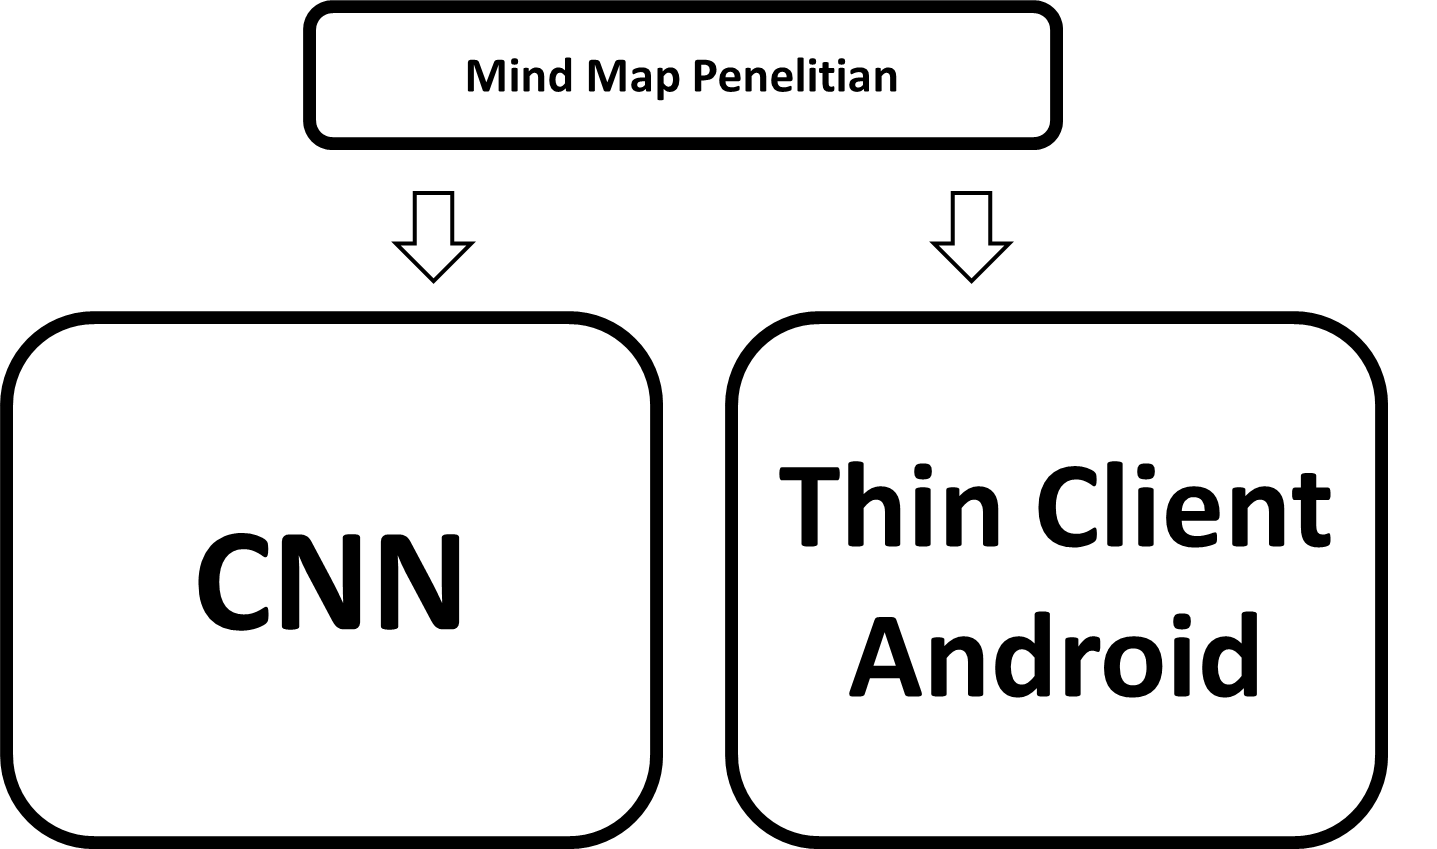
\includegraphics[width=8cm]{pics/mind_map_final}
	\caption{Mind map penelitian terdahulu terkait CNN}
	\label{fig:mind_map}
\end{figure}

Dalam penelitian \cite{can_deep_learning} yang dilakukan Nicholas D. LanePetko Georgiev, membangun prototipe deep neural network pada lingkungan low-power yang melibatkan CPU dan DSP of a perangkat mobile SoC (System On Chip). Deep Neural Network digunakan melakukan deteksi aktivitas dan dilakukan perbandingan dengan teknik pembelajaran umum lainnya. Penelitian ini menemukan DNN mampu melakukan komputasi tanpa memberikan beban pada perangkat mobile dan mampu meningkatkan akurasi inferensi. Selain itu, ditemukan bahwa Deep Neural Network dapat dengan baik bekerja pada skala kelas inferensi yang lebih besar dan dipartisi secara fleksibel pada sumber daya perangkat mobile.

Dalam penelitian \cite{deepear} yang dilakukan oleh Nicholas Lane, Petko Georgiev dan Lorena Qendro, menyajikan DeepEar yang merupakan framework perangkat mobile audio pertama dengan metode Deep Neural Network pada sensor audio secara simultan. Penelitian ini membuktikan bahwa DeepEar layak digunakan pada perangkat mobile yang dibangun dengan cloud yang berjalan secara kontinyu dan menghabiskan sumber daya 6\% per hari.

Dalam penelitian \cite{early_Resource} yang dilakukan oleh Nicholas D. Lane, Sourav Bhattacharya, Petko Georgiev, Claudio Forlivesi dan Fahim Kawsar, meneliti perhitungan model deep learning (misalnya Convolutional Neural Network) pada perangkat mobile dan platform embedded. Penelitian ini bertujuan untuk mempelajari performa, kebutuhan sumber daya dan bottleneck pada perangkat mobile ketika melakukan proses deep learning. Hasil dari penelitian ini memberikan fondasi untuk melakukan optimasi pada metode deep learning agar bisa diintegrasikan dengan teknologi IoT, smartphone dan sistem wearable.

Dalam penelitian \cite{deepx} yang dilakukan oleh Nicholas D. Lane, Sourav Bhattacharya, Petko Georgiev, Claudio Forlivesi, Lei Jiao, Lorena Qendro, dan Fahim Kawsar, menyajikan desain dan implementasi DeepX, yang merupakan perangkat lunak akselerator untuk melakukan proses deep learning. DeepX menyediakan algoritma untuk melakukan kontrol sumber daya ketika melakukan proses deep learning dengan melakukan dekomposisi model jaringan kedalam beberapa unit. Arsitektur DeepX membuktikan proses deep learning dapat melakukan proses secara efisien pada perangkat prosesor mobile modern.

Dalam penelitian \cite{smart_to_deep} yang dilakukan oleh Sourav Bhattacharya dan Nicholas D. Lane, meneliti metode Restricted Boltzmann Machines (RBM) untuk melakukan deteksi aktivitas pada perangkat smartwatch. Penelitian ini menyertakan variasi aktivitas seperti mode transportasi, aktivitas fisik dan deteksi dalam atau luar ruangan. Penelitian ini menunjukan Restricted Boltzmann Machines (RBM) dapat menggunakan sumber daya dan memungkinkan penggunaan deep learning pada perangkat smartwatch.

Dalam penelitian \cite{fast_rcnn} yang dilakukan oleh Ross Girshick, menciptakan metode deep learning Fast R-CNN yang merupakan penggabungan dari Region Convolutional Neural Network dan Spatial pyramid pooling networks (SPPnets). Penelitian ini bertujuan untuk memperbaiki kekurangan waktu proses R-CNN dan SPPnets pada saat training dan deteksi objek yang disebabkan multi-stage pipeline. Penelitian ini memberikan kontribusi perbaikan R-CNN dengan memberikan State-of-the-art mAP untuk VOC07, 2010, and 2012, waktu komputasi pembelajaran dan training yang lebih cepat dibandingkan R-CNN dan SPPnet dan fine-tune layer konvolusi.

Penelitian-penelitian terdahulu yang telah dijelaskan di atas dapat dituliskan dalam sebuah matriks literatur yang dapat dilihat pada \ref{tab:tab1} sebagai berikut.
\begin{table}
	\clearpage
	\centering
	\caption{Matriks literatur penelitian terdahulu yang berhubungan dengan penelitian Convolution Neural Network}
	\label{tab:tab1}
	\begin{tabular}{ |m{2cm}|m{7cm}|m{1cm}|m{1cm}| } 	
		\hline	
		Judul & \multicolumn{3}{|m{13cm}|}{Can Deep Learning Revolutionize Mobile Sensing} \\
		\hline
		Pengarang & \multicolumn{3}{|m{13cm}|}{Nicholas D. Lane \& Petko Georgiev} \\ 
		\hline
		Tahun & \multicolumn{3}{|m{13cm}|}{2015} \\ 
		\hline
		Metode & \multicolumn{3}{|m{13cm}|}{Implementasi Deep Neural Network pada soc mobile dan DSP (Digital Signal Processor)}\\
		\hline
		Kontribusi  & \multicolumn{3}{|m{13cm}|}{Implementasi Deep Learning dengan memanfaatkan sensor mobile}\\ 
		\hline
		Pekerjaan Mendatang  & \multicolumn{3}{|m{13cm}|}{Inovasi sensor mobile dengan deep learning} \\
		\hline\hline
		Judul & \multicolumn{3}{|m{13cm}|}{DeepEar: Robust Smartphone Audio Sensing in Unconstrained Acoustic Environments using Deep Learning} \\
		\hline
		Pengarang & \multicolumn{3}{|m{13cm}|}{Nicholas D. Lane, Petko Georgiev, Lorena Qendro} \\ 
		\hline
		Tahun & \multicolumn{3}{|m{13cm}|}{2015} \\ 
		\hline
		Metode & \multicolumn{3}{|m{13cm}|}{Implementasi Deep Neural Network untuk sensor audio pada mobile}\\
		\hline
		Kontribusi  & \multicolumn{3}{|m{13cm}|}{Implementasi deep learning untuk sensor audio pada mobile dan arsitektur yang memberikan efisiensi pada konsumsi power mobile}\\ 
		\hline
		Pekerjaan Mendatang  & \multicolumn{3}{|m{13cm}|}{Pengembangan sensor audio mobile untuk pengenalan aktivitas} \\
		\hline
		\hline\hline
		Judul & \multicolumn{3}{|m{13cm}|}{An Early Resource Characterization of Deep Learning on Wearables, Smartphones and Internet-of-Things Devices} \\
		\hline
		Pengarang & \multicolumn{3}{|m{13cm}|}{Nicholas D. Lane, Sourav Bhattacharya, Petko Georgiev, Claudio Forlivesi, Fahim Kawsar} \\ 
		\hline
		Tahun & \multicolumn{3}{|m{13cm}|}{2015} \\ 
		\hline
		Metode & \multicolumn{3}{|m{13cm}|}{Implementasi deep learning pada mobile dan platform embedded untuk meneliti performansi dan kebutuhan sumber daya mobile}\\
		\hline
		Kontribusi  & \multicolumn{3}{|m{13cm}|}{Metode fondasi metode deeplearning untuk teknologi IoT, smartphone and sistem wearable}\\ 
		\hline
		Pekerjaan Mendatang  & \multicolumn{3}{|m{13cm}|}{Pengembangan lanjut deeplearning pada IoT dan sistem wearable} \\
		\hline\hline
		Judul & \multicolumn{3}{|m{13cm}|}{DeepX: A Software Accelerator for Low-Power Deep Learning Inference on Mobile Devices} \\
		\hline
		Pengarang & \multicolumn{3}{|m{13cm}|}{Nicholas D. Lane, Sourav Bhattacharya, Petko Georgiev, Claudio Forlivesi, Lei Jiao, Lorena Qendro dan Fahim Kawsar} \\ 
		\hline
		Tahun & \multicolumn{3}{|m{13cm}|}{2016} \\ 
		\hline
		Metode & \multicolumn{3}{|m{13cm}|}{Dekomposisi model arsitektur deep learning menjadi beberapa blok unit dan pengaturan sumber daya model deep learning}\\
		\hline
		Kontribusi  & \multicolumn{3}{|m{13cm}|}{Optimasi sumber daya model deep learning untuk mobile}\\ 
		\hline
		Pekerjaan Mendatang  & \multicolumn{3}{|m{13cm}|}{Implementasi arsitektur DeepX pada mobile dengan variasi metode deep learning} \\
		\hline
	\end{tabular}
\end{table}

\begin{table}
	\clearpage
	\centering
	\begin{tabular}{ |m{2cm}|m{7cm}|m{1cm}|m{1cm}| } 	
		\hline	
		Judul & \multicolumn{3}{|m{13cm}|}{Fast R-CNN} \\
		\hline
		Pengarang & \multicolumn{3}{|m{13cm}|}{Ross Girshick} \\ 
		\hline
		Tahun & \multicolumn{3}{|m{13cm}|}{2015} \\ 
		\hline
		Metode & \multicolumn{3}{|m{13cm}|}{Integrasi dan optimasi Region-CNN dan Spatial pyramid pooling networks}\\
		\hline
		Kontribusi  & \multicolumn{3}{|m{13cm}|}{optimasi Region-CNN dan Spatial pyramid pooling networks}\\ 
		\hline
		Pekerjaan Mendatang  & \multicolumn{3}{|m{13cm}|}{Peningkatan deteksi objek dengan perbaikan metode sparse object} \\
		\hline
	\end{tabular}
\end{table}
%-----------------------------------------------------------------------------%
\section{\f{Feedforward Neural Network}} \label{fnn}
%-----------------------------------------------------------------------------%
Di dalam \f{machine learning}, \f{artificial neural network} (ANN) adalah model yang terinspirasi oleh \f{neural network} biologis. \f{Aritificial neural network} dapat melakukan estimasi atau aproksimasi fungsi non-linear dengan nilai \f{output} yang dapat berupa nilai \f{real}, diskret, atau vektor. Pada alamnya, neuron menerima sinyal melalui sinaps yang terletak pada dendrit. Neuron akan teraktivasi dan dapat meneruskan sinyal apabila sinyal yang diterima memenuhi batas tertentu. Sinyal tersebut dapat diterima sinaps lain dan dapat mengaktivasi neuron lainnya. Beberapa permasalahan yang dapat diselesaikan dengan ANN diantaranya adalah klasifikasi, kategorisasi, aproksimasi fungsi, dan prediksi .

\f{Feedforward neural network} adalah salah satu jenis ANN. \f{Feedforward neural network} terdiri dari beberapa unit yang dikelompokkan dalam \f{layer} di mana setiap \f{layer} yang bersebelahan saling terhubung melalui suatu unit. Pada \f{feedforward neural network}, koneksi antar \f{unit} tidak membentuk \f{cycle} seperti yang ada pada \f{recurrent neural network}. Kalkulasi \f{feedforward neural network} dari \f{input} ke \f{output} berjalan ke satu arah sesuai dengan strukturnya yang tampak seperti graf berarah. Contoh \f{feedforward neural network} dengan satu \f{hidden layer} dapat dilihat pada Gambar \ref{fig:fnn} berikut.

\begin{figure}
	\centering
	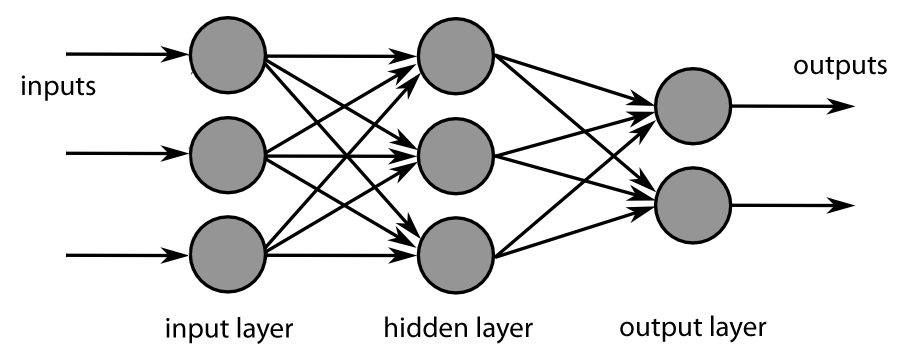
\includegraphics[width=0.8\textwidth,height=0.3\textwidth]
	{pics/fnn.png}
	\caption{Contoh \f{feedforward neural network}}
	\label{fig:fnn}
\end{figure}
\vspace{-1.2cm}
\begin{center}
	{\small Sumber gambar: http://technobium.com/stock-market-prediction-using-neuroph-neural-networks/}
\end{center}

\f{Feedforward neural network} terdiri dari \f{input layer}, \f{output layer}, dan beberapa \f{hidden layer} apabila dibutuhkan. Jumlah \f{hidden layer} berperan pada seberapa kompleks batas keputusan yang dapat dibentuk oleh \f{network} seperti pada Gambar \ref{fig:hl}.

\begin{figure}
	\centering
	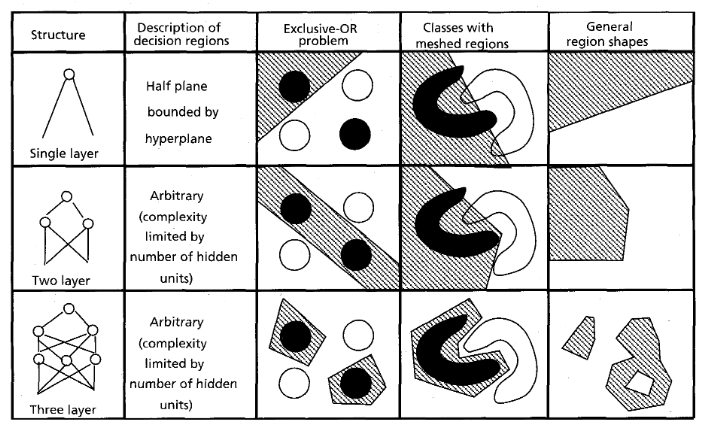
\includegraphics[width=1\textwidth,height=0.6\textwidth]
	{pics/hl.png}
	\caption{Interpretasi geometris pada peran \f{hidden layer}}
	\label{fig:hl}
\end{figure}
\vspace{-1.2cm}
\begin{center}
	{\small Sumber gambar: \cite{paper.jain}}
\end{center}

Pada \f{input layer}, jumlah unit atau neuron yang ada sesuai dengan jumlah elemen yang ada pada vektor \f{input}. Begitu juga dengan \f{output layer}, jumlah unit yang ada sesuai dengan banyaknya elemen yang diinginkan pada vektor \f{output}. Berbeda dengan \f{input layer} dan \f{output layer}, jumlah unit dalam \f{hidden layer} sifatnya bebas. Setiap unit menghasilkan suatu \f{output} dari kombinasi linear beberapa nilai \f{input} dengan bobotnya masing-masing. Hasil dari kombinasi linear tersebut kemudian diaktivasi dengan fungsi aktivasi. Proses ini dapat dilihat pada Rumus \ref{equ:perceptron}.

\begin{equation}
\label{equ:perceptron}
y(x) = g\left(\sum\limits_{i=1}^{n} w_{ij}x_{i} + w_{0j}\right)
\end{equation}

\begin{itemize}
	\item $x$ merupakan vektor \f{input}
	\item $w$ merupakan vektor bobot
	\item $w_{ij}$ merupakan bobot yang menghubungkan unit ke-\f{i} pada \f{layer} sebelumnya dan unit ke-\f{j} pada \f{layer} saat itu
	\item $w_{0j}$ merupakan bobot untuk bias
	\item $g$ merupakan fungsi aktivasi
\end{itemize}

Pada Rumus \ref{equ:perceptron} vektor \f{input} pada suatu \f{layer} bergantung pada \f{output} di \f{layer} sebelumnya, kecuali untuk \f{layer} pertama yaitu \f{input layer}. Fungsi aktivasi $g$ dapat berbeda untuk setiap \f{layer}, tapi pada umumnya sama untuk setiap unit pada \f{layer} yang sama. Pada penelitian ini fungsi aktivasi yang digunakan adalah \f{rectified linear unit} (ReLU) yang dapat dilihat pada Rumus \ref{equ:relu}, dan \f{sigmoid} pada Rumus \ref{equ:sigmoid}.

\begin{equation}
\label{equ:relu}
g(x) = max(0, x)
\end{equation}

\begin{equation}
\label{equ:sigmoid}
g(x) = \frac{1}{1 + e^{-x}}
\end{equation}

Pada Rumus \ref{equ:perceptron} terdapat $w_{0j}$ yang merupakan bobot untuk bias. Bias bersifat seperti konstanta yang selalu bernilai +1, sehingga pengaruh bias tergantung pada bobotnya.

%-----------------------------------------------------------------------------%
\section{Convolution Neural Network (CNN)}
%-----------------------------------------------------------------------------%
CNN merupakan salah satu variasi dari multilayer perceptron (MLP). Keuntungan dari metode CNN, khsusnya untuk kasus pengenalan pola dibandingkan pendekatan konvensional adalah kemampuan untuk mengurangi dimensi data, ekstraksi fitur secara sekuensial, dan mengklasifikasi salah satu struktur jaringan. Arsitektur dasar dari model CNN terinspirasi dari visual cortex yang dikenalkan oleh hubel dan wiesel pada tahun 1962.

Pada tahun 1980, neocognitron fukushima membuat pertama kali komputasi menggunakan model CNN, dan kemudian pada tahun 1989, dengan menggunakan model yang ditemukan fukushima, LeCun menemukan performa dari beberapa proses untuk pengenalan pola menggunakan metode error gradient.

Model CNN yang digunakan oleh LeCun merupakan pengembangan dari MLP tradisional yang didasari 3 ide, local receptive field, weight sharing dan spatial subsampling. Ide dasar ini diorganisir kedalam 2 tipe layer, yaitu convolution dan subsampling layer. Seperti yang ditunjukan gambar 1, digunakan 3 convolution layer dengan kombinasi layer subsampling dan 1 output layer. Layer convolution dan subsampling tersusun kedalam plane atau disebut feature maps.

\f{Convolutional neural network} (CNN) adalah salah satu tipe \f{feedforward neural network} yang terinspirasi dari cara kerja visual korteks. Berdasarkan penelitian , korteks visual terdiri dari banyak sel kompleks. Sel-sel ini disebut \f{receptive field} dan sensitif terhadap bagian kecil bidang visual. Salah satu sifat yang dimiliki CNN adalah \f{sparse connectivity}. \f{Sparse connectivity} memungkinkan suatu \f{layer} saling terhubung hanya dengan unit-unit terdekat. Dengan kata lain, \f{input} dari suatu unit merupakan \f{subset} dari unit pada \f{layer} sebelumnya. Ilustrasi \f{sparse connectivity} dapat dilihat pada Gambar.

\begin{figure}
	\centering
	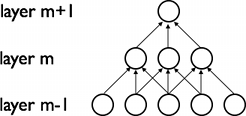
\includegraphics[width=0.45\textwidth,height=0.2\textwidth]
	{pics/sparse.png}
	\caption{\f{Sparse Connectivity}}
	\label{fig:sparse}
\end{figure}
\vspace{-1.2cm}
\begin{center}
	{\small Sumber gambar: http://deeplearning.net/tutorial/lenet.html}
\end{center}

Tumpukan \f{layer} pada Gambar \ref{fig:sparse} hanya memiliki satu unit pada \f{layer} $m + 1$. Hal ini merepresentasikan unit atau bagian-bagian kecil yang ada pada \f{layer} $m - 1$ bagaikan disaring atau di-\f{filter} hingga \f{layer} $m + 1$ memahami bidang visual secara utuh. 

Selain \f{sparse connectivity}, CNN juga memiliki sifat \f{shared weights}. Setiap \f{layer} kecuali \f{output layer} memiliki \f{filter} yang fungsinya untuk menyaring bagian kecil dari bidang visual. \f{Filter} tersebut direplikasi dengan bobot yang sama ke seluruh bidang visual dengan untuk menyaring unit atau bagian-bagian kecil sehingga membentuk \f{feature map}. Pada Gambar \ref{fig:shared} berikut, lima unit pada \f{layer} $m - 1$ disaring dengan \f{filter} berukuran tiga, sehingga membentuk tiga unit \f{feature map}. Garis yang berwarna sama menandakan bobot yang sama.

\begin{figure}
	\centering
	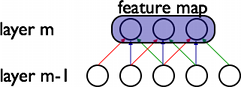
\includegraphics[width=0.45\textwidth,height=0.15\textwidth]
	{pics/shared.png}
	\caption{\f{Shared weights} untuk \f{filter} yang sama}
	\label{fig:shared}
\end{figure}
\vspace{-1.2cm}
\begin{center}
	{\small Sumber gambar: http://deeplearning.net/tutorial/lenet.html}
\end{center}

Untuk merepresentasikan data atau bidang visual yang kompleks, setiap \f{layer} pada CNN dapat mempunyai beberapa \f{feature map} atau \f{channel}. Rumus untuk menghitung \f{feature map} ke-$k$ pada \f{pixel} koordinat $(i,j)$ yang ditentukan oleh bobot $W^{k}$ dan bias $b_{k}$ adalah sebagai berikut.

\begin{equation}
\label{equ:featuremap}
y^{k}_{ij} = g\left((W^{k} * x)_{ij} + b_{k}\right)
\end{equation}

Setiap \f{feature map} pada layer $m - 1$ berkontribusi dalam menentukan nilai \f{feature map} $k$ pada layer $m$. Dengan kata lain, setiap \f{pixel} yang berada dalam \f{feautre map} $k$ nilainya akan ditentukan oleh seluruh \f{pixel} yang terhubung, pada \f{feature map} di \f{layer} $m - 1$. Pada ilsutrasi Gambar \ref{fig:featuremap}, \f{layer} $m$ memiliki dua \f{feature map} $y^0$ dan $y^1$. \f{Pixel} (kotak berwarna biru) pada $y^0$ ditentukan dari 2x2 \f{pixel} yang terhubung dengan bobot $W^{kl}_{ij}$. $W^{kl}_{ij}$ menyatakan bobot yang menghubungkan \f{pixel} koordinat $(i,j)$ pada \f{feature map} ke-$l$ di \f{layer} $m - 1$ ke \f{pixel} yang terhubung pada \f{feature map} ke-$k$ di \f{layer} $m$.

\begin{figure}
	\centering
	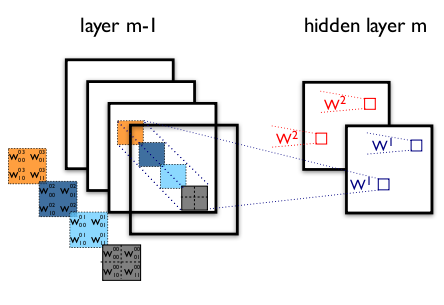
\includegraphics[width=0.9\textwidth,height=0.55\textwidth]
	{pics/featuremap.png}
	\caption{Ilustrasi \f{layer} pada \f{convolutional neural network}}
	\label{fig:featuremap}
\end{figure}
\vspace{-1.2cm}
\begin{center}
	{\small Sumber gambar: http://deeplearning.net/tutorial/lenet.html}
\end{center}

\f{Convolutional Neural Network} biasanya terdiri dari beberapa \f{filter} atau disebut juga dengan \f{convolutional layer}, sering kali diikuti denga \f{subsampling layer} dan diakhiri dengan \f{fully connected layers}. Terdapat juga jenis CNN yang tidak diakhiri dengan \f{fully connected layers} melainkan \f{convolutional layer} lainnya yang mempertahankan dimensi data dalam bentuk citra 2D. CNN jenis ini disebut dengan \f{Fully Convolutional Neural Network}.

\subsection{Convolutional Layer}
Pada layer convolution, tiap neuron terhubung secara local kepada area yang lebih kecil (local receptive field) pada layer sebelumnya. Semua neuron yang memiliki feature maps yang sama memperoleh data dari input area yang berbeda hingga semua input plan tersaring tetapi saling berbagi bobot (weight sharing).\\
\f{Convolutional layer} memiliki tiga \f{hyperparameter} yang mengatur transformasi \f{feature map} yang dihasilkan: \f{depth} $D$, \f{stride} $S$, dan \f{zero-padding} $P$. Dalam tahap \f{feedforward}, \f{convolutional layer} berukuran $F$ akan bergeser pada gambar berukuran $W$, dan menghasilkan \f{feature map} sebanyak $D$ dengan ukuran $W'$ yang dapat dihitung menggunakan Rumus \ref{equ:convlayer} berikut.

\begin{equation}
\label{equ:convlayer}
W' = (W - F + 2P) / S + 1
\end{equation}

Dalam praktiknya, \f{zero-padding} sering kali digunakan untuk menyesuaikan ukuran hasil \f{feature map}. \f{Zero padding} dengan ukuran $P = (F - 1)/2$ dipastikan menghasilkan \f{feature map} dengan ukuran yang sama dengan \f{feature map} sebelumnya apabila \f{stride} $S = 1$. \f{Deep learning framework} seperti \f{theano} menyebut \f{padding} dengan sifat tersebut sebagai \f{same padding} . Terdapat juga \f{full padding} yang menghasilkan \f{feature map} dengan ukuran $W' = W + F - 1$.

\subsection{Subsampling Layer}
Pada layer subsampling, feature maps didownsampling secara spasial, dimana ukuran map dikurangi berdasarkan 2 faktor. Contohnya, feature map pada layer C3 dengan ukuran 10x10 dilakukan subsampling untuk menyesuaikan feature map dengan ukuran 5x5 pada layer selanjutnya. Layer terakhir adalah F6 yang merupakan proses klasifikasi.
Dalam arsitektur \f{convolutional neural network}, \f{pooling layer} berfungsi untuk mereduksi ukuran spasial gambar secara bertahap sehingga mengurangi parameter dan komputasi pada \f{network}. \f{Pooling layer} menerima \f{input} \f{feature map} berukuran $W_{1}$ sebanyak $D_{1}$ dan parameter ukuran \f{pooling} $F$ dan \f{stride} $S$. Sama halnya dengan \f{convolutional layer}, \f{pooling layer} juga bergeser terhadap input dan menghasilkan \f{feature map} berjumlah $D_{2} = D_{1}$ dengan ukuran $W_{2} = (W_{1} - F)/S + 1$. Terdapat beberapa jenis \f{pooling layer}, dan yang paling sering digunakan adalah:

\begin{enumerate}
	\item \f{Max Pooling} \\
	Dalam \f{pooling} berukuran $F$, \f{Max pooling} akan mengambil hasil aktivasi yang terbesar dalam daerah yang termasuk pada pergeseran saat itu. Ilustrasi ini dapat dilihat pada Gambar \ref{fig:maxpool} berikut dengan $F = 2$ dan $S = 2$.
	
	\begin{figure}
		\centering
		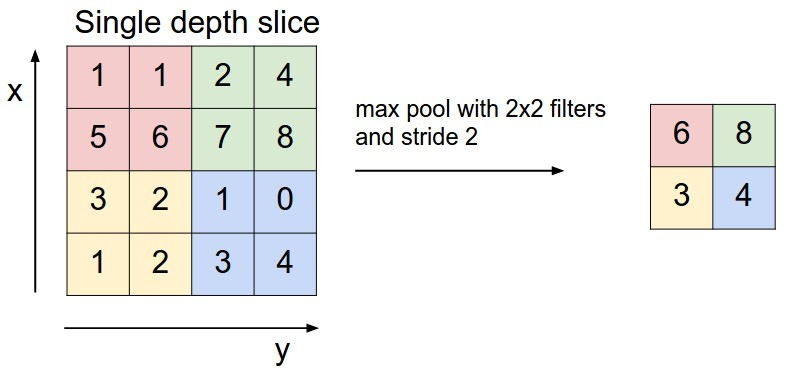
\includegraphics[width=0.8\textwidth,height=0.35\textwidth]
		{pics/maxpool.jpeg}
		\caption{Ilustrasi \f{max pooling}}
		\label{fig:maxpool}
	\end{figure}
	\vspace{-1.2cm}
	\begin{center}
		{\small Sumber gambar: http://cs231n.github.io/convolutional-networks}
	\end{center}
	
	\item \f{Average Pooling} \\
	Berbeda dengan \f{max pooling}, \f{average pooling} mengambil hasil aktivasi pada daerah \f{filter} dan menghitung rata-rata dari seluruh hasil aktivasi dalam daerah tersebut.
\end{enumerate}
%-----------------------------------------------------------------------------%
\subsection{\f{Fully Connected Layer}}
%-----------------------------------------------------------------------------%
\f{Fully connected layer} adalah \f{feed forward neural network} yang dijelaskan pada subbab \ref{fnn}. Biasanya, \f{fully connected layer} berada pada \f{layer} akhir pada arsitektur \f{convolutional neural network} dan bertujuan untuk memproses hasil \f{feature extraction} yang dilakukan pada \f{layer} sebelumnya menjadi suatu \f{output} tertentu. Gambar \ref{fig:cnnlayers} berikut merupakan contoh arsitektur dengan susunan \f{convolutional layer}, \f{pooling layer}, dan \f{fully connected layer}.

\begin{figure}
	\centering
	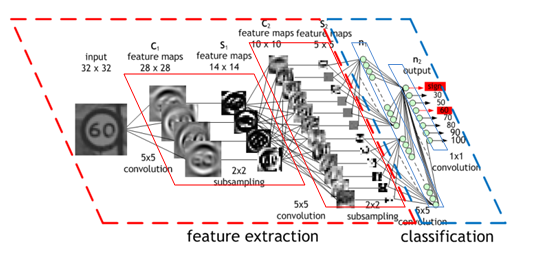
\includegraphics[width=1\textwidth,height=0.45\textwidth]
	{pics/cnnlayers.png}
	\caption{Contoh arsitektur \f{convolutional neural network}}
	\label{fig:cnnlayers}
\end{figure}
\vspace{-1.2cm}
\begin{center}
	{\small Sumber gambar: https://devblogs.nvidia.com}
\end{center}
%-----------------------------------------------------------------------------%
\section{\f{Backpropagation}}
%-----------------------------------------------------------------------------%
Tujuan dari melatih model \f{feedforward neural network} adalah membuat model tersebut dapat memprediksi nilai dengan galat seminimal mungkin. \f{Feedforward neural network} menggunakan metode \f{backpropagation} untuk melatih nilai bobot-bobot pada \f{network} tersebut. Untuk melatih suatu bobot, metode ini melakukan \f{propagation} dari galat pada \f{output layer} sehingga informasi ini tersebar ke \f{layer} sebelumnya untuk digunakan dalam mengubah bobot.

Untuk $\delta^{(l+1)}$ sebagai galat pada \f{layer} $l+1$ dengan fungsi galat $J(W,b;x,y)$ di mana $W,b$ adalah parameter, dan $x,y$ adalah pasangan \f{input} dan label, apabila \f{layer} $l$ dan \f{layer} $l+1$ saling terhubung maka galat pada \f{layer} $l$ adalah sebagai berikut.


\begin{equation}
\begin{aligned}
\delta^{(l)} &= ((W^{(l)})^{T}\delta^{(l+1)}) \cdot f'(z^{(l)}) \\
f'(z^{(l)}) &= a^{(l)} \cdot (1-a^{(l)})
\end{aligned}
\end{equation}

\begin{equation}
\label{equ:erder}
\begin{aligned}
\Delta_{w^{(l)}}J(W,b;x,y)&=\delta^{(l+1)}(a^{(l)})^{T} \\
\Delta_{b^{(l)}}J(W,b;x,y)&=\delta^{(l+1)}
\end{aligned}
\end{equation}

Pada \f{convolutional layer} dan \f{pooling layer}, galat pada \f{layer} $l$ dihitung dengan fungsi \f{upsample} $g(x)$ tergantung pada \f{layer} yang digunakan.

\begin{equation}
\label{equ:errorc}
\delta^{(l)}_{k} = upsample((W^{(l)}_{k})^{T}\delta^{(l+1)}_{k}) \cdot f'(z^{(l)}_{k}) 
\end{equation}

\[
g(x)
\begin{cases}
\frac{\sum_{k=1}^{m} x_{k}}{m}, \frac{\delta g}{\delta x} = \frac{1}{m}, & \text{average pooling} \\
max(x), \frac{\delta g}{\delta x} =
\begin{cases}
1, & \text{if } x_{i} = max(x) \\
0, & otherwise
\end{cases}
, & \text{max pooling}
\end{cases}
\]

\begin{center}
	{\small Sumber rumus: http://www.slideshare.net/kuwajima/cnnbp}
\end{center}

Rumus \ref{equ:erder} digunakan untuk mengubah bobot pada suatu \f{layer}. Salah satu cara untuk mengubah bobotnya adalah dengan \f{stochastic gradient descent} yang menggunakan Rumus \ref{equ:sgd} berikut.

\begin{equation}
\label{equ:sgd}
\theta = \theta-\alpha\Delta_{\theta}J(\theta;x^{(i)},y^{(i)})
\end{equation}

\begin{center}
	{\small Sumber rumus: http://ufldl.stanford.edu/tutorial/supervised/ConvolutionalNeuralNetwork}
\end{center}


%-----------------------------------------------------------------------------%
\section{Algoritma Optimasi}
%-----------------------------------------------------------------------------%
Algoritma optimasi digunakan untuk permasalahan meminimalisasi \f{loss}. Untuk \f{dataset} $D$, objektif dari optimasi adalah rata-rata $loss$ $|D|$ dari seluruh anggota \f{dataset} $D$. Dengan $fw(X^{(i)})$ adalah galat pada data ke $X^{(i)}$, dan $r(W)$ adalah regularisasi dengan bobot $\lambda$, maka galat rata-rata dapat dihitung menggunakan Rumus \ref{equ:avgloss} berikut .

\begin{equation}
\label{equ:avgloss}
L(W)=\frac{1}{|D|}\sum\limits_{i}^{|D|}fw(X^{(i)})+\lambda r(W)
\end{equation}

Karena $|D|$ pada kenyataannya dapat bernilai sangat besar, dalam praktiknya setiap iterasi menggunakan aproksimasi secara stokastik dengan memilih $N << |D|$ sehingga galat rata-rata dihitung dengan Rumus \ref{equ:avgloss2} berikut .

\begin{equation}
\label{equ:avgloss2}
L(W)\approx\frac{1}{N}\sum\limits_{i}^{N}fw(X^{(i)})+\lambda r(W)
\end{equation}
%-----------------------------------------------------------------------------%
\subsection{\f{Stochastic Gradient Descent} (SGD)}
%-----------------------------------------------------------------------------%
\f{Stochastic gradient descent} mengubah bobot $W$ dengan kombinasi linear dari \f{gradient} negatif $\Delta L(W)$ dan perbaharuan bobot $V_{t}$ pada iterasi sebelumnya. Untuk menghitung nilai perbaharuan $V_{t+1}$ dan bobot $W_{t+1}$ pada iterasi $t+1$ digunakan Rumus \ref{equ:sgd2} dan \ref{equ:sgd2-3} berikut .

\begin{equation}
\label{equ:sgd2}
V_{t+1} = \mu V_{t} - \alpha \Delta L(W_{t})
\end{equation}

\begin{equation}
\label{equ:sgd2-3}
W_{t+1} = W_{t} + V_{t+1}
\end{equation}
%-----------------------------------------------------------------------------%
\subsection{\f{Nesterov's Accelerated Gradient} (Nesterov)}
%-----------------------------------------------------------------------------%
\f{Nesterov's accelerated gradient} (Nesterov) diusulkan oleh Nesterov sebagai metode optimal untuk optimasi, dengan laju konvergensi mencapai $O(1/t^{2})$. Dalam praktiknya, Nesterov dapat menjadi metode yang cukup efektif untuk mengoptimasi arsitektur \f{deep learning} tertentu, seperti yang didemonstrasikan oleh  dalam membuat \f{autoencoders}. Perubahan bobot dalam algoritma Nesterov menggunakan Rumus berikut .

\begin{equation}
\label{equ:nesterov}
V_{t+1}=\mu V_{t} - \alpha\Delta L(W_{t} + \mu V_{t})
\end{equation}

\begin{equation}
W_{t+1} = W_{t} + V_{t+1}
\end{equation}

Perbedaan Nesterov dengan SGD terdapat pada penambahan momentum dalam menghitung \f{gradient} $\Delta L(W_{t} + \mu V_{t})$. Dalam SGD, perhitungan \f{gradient} $\Delta L(W_{t})$ hanya mengambil bobotnya saja.

%-----------------------------------------------------------------------------%
\section{Fungsi Galat}
%-----------------------------------------------------------------------------%
Fungsi galat adalah fungsi yang menghitung galat dari hasil prediksi $\hat{y}$ dengan nilai $y$ yang sebenarnya. Pada penelitian ini, penulis menggunakan dua jenis fungsi galat, yakni \f{cross-entropy loss} (Rumus \ref{equ:cl}) dan \f{euclidean loss} (L2) (Rumus \ref{equ:el}). Dilihat dari fungsinya, \f{cross entropy} bekerja lebih agresif dalam memperbaiki dibandingkan dengan \f{euclidean error}.

\begin{equation}
\label{equ:cl}
crossentropy(y, \hat{y}) = -(y * log(\hat{y}) + (1 - y) * log(1 - \hat{y}))
\end{equation}

\begin{equation}
\label{equ:el}
euclideanloss(y, \hat{y}) = \frac{1}{2} \|y - \hat{y}\|^{2}_{2}
\end{equation}
\begin{center}
	{\small Sumber rumus: http://caffe.berkeleyvision.org}
\end{center}
%-----------------------------------------------------------------------------%
\section{Fast R-CNN}
%-----------------------------------------------------------------------------%

Arsitektur Fast R-CNN \ref{fig:arsitektur_fcnn} memiliki input objek gambar dan gambar yang sudah diberikan RoI (Object Proposal). Input akan diproses pertama kali kedalam beberapa layer konvolusi dan max pooling untuk mendapatkan feature map. Kemudian tiap objek proposal dengan Region of Interest (RoI) akan melakukan ekstraksi fitur dari feature map. Tiap vektor dari fitur akan diproses secara berurutan kedalam Fully Connected Layer dan dipecah ke dalam 2 output layer. Layer pertama menggunakan probabilitas softmax untuk melakukan estimasi pada K kelas object dan background. Layer kedua memberikan 4 output dalam bentuk bilangan real untuk tiap K kelas objek. Untuk setiap 4 nilai dilakukan encoding posisi bounding-box pada salah satu posisi dari kelas K.

\begin{figure}[htp]
	\centering
	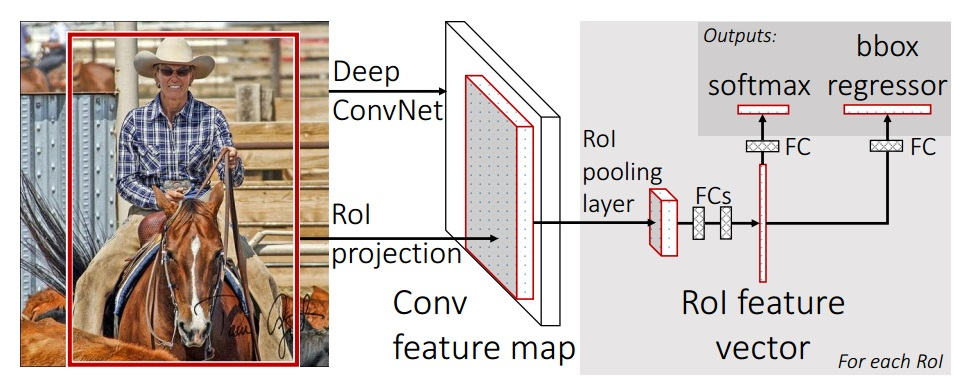
\includegraphics[width=10cm]{pics/arsitektur_fcnn}
	\caption{Arsitektur Fast R-CNN}
	\label{fig:arsitektur_fcnn}
\end{figure}

\subsection{RoI pooling layer}
RoI merupakan suatu area yang berbentuk segi empat dan berada didalam feature map konvolusi. Layer RoI pooling bertujuan melakukan proses max pooling dengan tujuan konversi fitur didalam RoI kedalam feature map yang lebih kecil dengan ukuran yang sudah didefinisikan sebelumnya. RoI didefinisikan menggunakan 4 tuple \f{(r, c, h, w)} dimana \f{(r, c)} mendefinisikan \f{top-left corner} dan \f{(h, w)} mendefinisikan nilai tinggi dan lebar.

Proses max poling pada ROI membagi area dengan \f{h x w} menjadi \f{H x W} sub-window dengan rumus \f{h/H x w/W}. Nilai sub-windows tersebut akan memiliki korespondensi dengan output grid cell. Pooling dilakukan secara independen kepada tiap channel feature map yang merupakan standard dari max pooling.

\subsection{Pre-trained networks}
Pada \cite{fast_rcnn}, pra pembelajaran jaringan menggunakan 5 layer max pooling dan layer konvolusi dengan jumlah antara 5 hingga 13 layer dengan data training. Pra pembelajaran jaringan bertujuan memberikan inisialisasi Fast R-CNN dengan melakukan 3 transformasi:
\begin{enumerate}
	\item Layer max pooling terakhir dirubah menjadi layer RoI pooling yang dikonfigurasi dengan \f{H} dan \f{W} agar sesuai dengan layer Fully Connected pertama.
	\item Layer Fully Connected dan softmax terakhir dirubah menjadi 2 layer output
	\item Network dimodifikasi kedalam 2 input data: input gambar dan RoI pada tiap input gambar tersebut.
\end{enumerate}

\subsection{\f{Fine-tuning} untuk Deteksi}
Fast R-CNN memiliki metode training yang efisien dengan memanfaatkan sharing feature. Minibatch Stochastic Gradient Descent (SGD) dilakukan proses sampling secara hirarki, yaitu N gambar dan dilakukan secara iterarif \f{R/N} dari tiap gambar. RoI dari gambar yang sama akan menggunakan komputasi dan memori pada proses forward dan backward. Contohnya, ketika N=2 dan R=128, skema training akan meningkat 64x kali lebih cepat dibandingkan menggunakan 1 RoI dengan 128 gambar. Salah satu permasalahan pada skema training ini adalah proses training akan berjalan lambat karena RoI dari gambar yang sama akan saling berkorelasi. Berdasarkan \cite{fast_rcnn}, masalah ini tidak menjadi isu pada saat pembelajaran dan tetap memberikan hasil yang baik karena jumlah iterasi SGD yang lebih sedikit dibandingkan R-CNN biasa.

Sebagai tambahan pada proses sampling yang dilakukan secara hirarki, Fast R-CNN menggunakan proses training yang lebih singkat dengan fase \f{fine-tuning} yang menggabungkan softmax dan bounding-box regressor, dibandingkan R-CNN biasa yang melakukan training dengan softmax, SVM dan regressor pada fase yang berbeda. Detail komponen \f{fine-tuning} sbb:
\begin{itemize}
	\item Multi-task loss\\
	Fast R-CNN memiliki 2 output layer: layer pertama memberikan output distribusi probabilitas diskret, \f{p = ($p\sb{0}$, . . . , $p\sb{K}$)}, per $K+1$ kategori. Kemudian $p$ dihitung menggunakan softmax pada output $K+1$ dari layer Fully Connected. Layer kedua memberikan output bounding-box regression offset, $tk = t^k_x , t^k_y , t^k_w, t^k_h$, untuk tiap $K$ kelas objek, menggunakan index $k$. $tk$ didesinisikan meenggunakan translasi scale-invariant dan log-space pergeseran tinggi atau lebar menyesuaikan proposal objek.
	
	Setiap melakukan training RoI akan diberi label kelas $u$ dan target bounding-box regression $v$. Fast R-CNN menggunakan multi-task loss $L$ pada tiap RoI yang sudah memiliki label untuk dilatih proses klasifikasi dan regression bounding-box

	\begin{equation}
	\label{equ:fcnn_reg_bounding_box}
	L(p, u, t^u, v) = L\sb{cls}(p, u) + λ[u ≥ 1]L\sb{loc}(t^u, v)
	\end{equation}
	
	dimana $L\sb{cls}(p, u) = -log p_u$ merupakan log loss dari kelas $u$ true. $L\sb{loc}$ didefinisikan pada tuple dari true target bounding-box regression pada kelas $u, v = (v_x, v_y, v_w, v_h)$, dan tuple $tu = (t^u_x , t^u_y , t^u_w, t^u_h)$ untuk kelas $u$. Indikator kurung iverson $[u ≥ 1]$ dievaluasi menjadi 1 ketika $u ≥ 1$ dan 0 sebagainya. Dengan syarat pengambilan semua kelas background diberikan label 0. Untuk background RoI tidak ada gagasan sehingga $L\sb{loc}$ diabaikan. Untuk bounding-box regression, digunakan fungsi loss

	\begin{equation}
	\label{equ:bounding_box_regression}
		L\sb{loc}(t^u, v) = \sum_{i∈{x,y,w,h}} smooth\sb{L_1}(t^u_i − v_i)
	\end{equation}

	dimana

	\begin{equation}
	\label{equ:rumus_3}	
smooth\sb{L_1}(x) = 
\begin{cases}
0.5x^2 & \text{ jika x < 1} \\
|x| - 0.5 & \text{otherwise} 
\end{cases}
\end{equation}
	
	adalah loss $L_1$ yang tidak terlalu sensitif pada outlier dibandingkan loss $L_2$ yang digunakan R-CNN dan SPPnet. Ketika target regresi tidak memiliki batas, training $L_2$ akan membutuhkan perbaikan pada learning rate dengan tujuan mencegah perubahan gradien. Rumus \ref{equ:rumus_3} menghilangkan sensitifitas ini.
	\item Mini-batch sampling\\
	Selama melakukan fine-tuning, tiap mini-batch SGD dibangun dengan gambar $N = 2$ , yang dipilih secara acak. Ukuran mini-batch yang digunakan $R = 128$, dengan melakukan sampling 64 RoI dari tiap gambar. Roi yang diambil hanya 25\% dari objek proposal ketika terjadi saling tumpuk dengan batas 0.5 pada bounding box. RoI mengandung contoh yang diberikan label dengan kelas object foreground yaitu $u \geq 1$. RoI sisanya akan dilakukan sampel dari objek proposal yang memiliki maksimum IoU dengan interval [0.1, 0.5].
	
	\item Back-propagation through RoI pooling layers\\
	Backpropagation mengarah pada penuruan pada layer pooling Roi. Untuk memperjelas, diasumsikan hanya 1 gambar per batch $(N = 1)$, perluasan pada $N > 1$ akan terang-terangan karena proses forward memperlakukan gambar secara independen.
	
	$x_i \in R$ menjadi input aktivasi $i$-th kedalam layer RoI pooling dan $y\sb{rj}$ menjadi bagian $j$-th memberikan output $r$-th RoI. Layer RoI pooling menghitung $y\sb{rj} = x\sb{i*(r,j)}$ dimana $i*(r,j) = argmax\sb{i' \in R(r,j)}x\sb{i'}$. $R(r, j)$ adalah kumpulan indeks dari input dalam sub-window dimana pada unit output $yrj$ max pool. Satu $x_i$ bisa diberikan kepada beberapa output $y\sb{rj}$. \\
	Proses backward Layer RoI pooling  menghitung turunan parsial dari loss function dengan untuk tiap variabel input $x_i$ sbb:
	
	\begin{equation}
	\label{equ:backward_roi_pooling}
	\frac{\partial L}{\partial x_i} = \sum_{r}^{}\sum_{j}^{}[i = i^* (r,j)] \frac{\partial L}{\partial y\sb{r,j}}
	\end{equation}
	
	Dengan kata lain, untuk setiap mini-batch RoI $r$ dan untuk setiap unit output pooling $y\sb{rj}$, dilakukan akumulasi penurunan parsial $\partial L/\partial y\sb{rj}$ jika $i$ adalah argmax yang terpilih untuk $y\sb{rj}$ dengan max pooling. pada backpropagation, penurunan parsial $\partial L/\partial y\sb{rj}$ sudah dihitung dengan fungsi backward dari layer teratas dari layer RoI pooling.
	
	\item SGD hyper-parameters\\
	Layer Fully Connected yang digunanakan untuk klasifikasi softmax dan regression bounding-box merupakan hasil inisialisasi dari distribusi zero-mean gaussian dengan standard deviasi 0.01 dan 0.01. Nilai bias diinisialisasi menjadi 0. Semua layer menggunakan learning rate bobot 1 dan 2 untuk bias dan learning rate global sejumlah 0.001. Momentum 0.9 dan parameter decay digunakan.
\end{itemize}

\subsection{Scale invariance}
Fast R-CNN mengeksplorasi 2 cara untuk memperoleh invarian ska deteksi objek: brute force dan menggunakan image piramid. Pendekatan Brute Forse, tiap gambar diproses dengan ukuran pixel yang belum didefinisikan selama proses training maupun testing. Network harus mempelajari langsung deteksi objek scale-invariant  dari data training. Pendekatan Multi-scale, berbanding terbalik, menyediakan pendekatan scala-invariance pada network pada image piramid. pada waktu tes, image piramid digunakan scale-normalize dari tiap objek proposal. selama multi-scale training, dipili secara acak skala piramida ketika image dijadikan sampel.

%-----------------------------------------------------------------------------%
\section{Thin Client Computing}
%-----------------------------------------------------------------------------%
Berdasarkan \cite{thin_client_computing}, Thin client merupakan istilah kepada komputer yang bersifat ringan dengan tujuan melakukan akses kepada server yang bersifat cloud maupun virtual. Kemunculan thin client disebabkan penggunaan komputer desktop yang memberikan beban dalam proses manajemen maupun maintenance.  Terminal services atau remote desktop services adalah salah satu software yang menyediakan fasilatas komunikasi dengan thin client, dimana biasanya pada suatu perusahaan akan membeli mesin thin client, melakukan instalasi microsoft windows server, kemudian dilakukan konfigurasi peraturan akses antara terminal service dan client dengan memberikan session untuk tiap komunikasi. Secara umum, penggunaan terminal service adalah salah satu solusi terbaik dan cocok untuk penggunaan aplikasi berskala kecil maupun penggunaan internal, harga terjangkau dan kemudahan proses instalasi dan maintenance. Selain terminal services, teknologi yang mampu mengadopsi thin client adalah CITRIX XENAPP.

Thin client berbasis desktop memiliki kekurangan yaitu dibutuhkannya mobilitas dari pengguna, pembaharuan pada hardware client, keamanan data dan beberapa kondisi tertentu yang perlu diperhatikan seperti konsumsi listrik dan pendinginan. Selain itu, perkembangan thin client saat ini mulai mengarah ada embedded desktop systems, menggunakan RAM dengan kapasitas tinggi, mendukung multi monitor, bahkan menggunakan teknologi smartphone yang saat ini perkembangannya sangat pesat dengan didukung komposisi hardware yang semakin mumpuni.

%-----------------------------------------------------------------------------%
\section{Teknologi Perangkat Mobile}
%-----------------------------------------------------------------------------%
\subsection{Sensor pada mobile}
Meskipun sensor pada perangkat mobile memiliki variasi dalam beberapa bentuk dan target untuk penggunaan secara umum, penggabungan elemen antara sensor adalah mereka semua melibatkan kumpulan dan interpretasi dari data. untuk menyelesaikan hal ini, mobile sensor mobile akan ditanaman algoritma deep learning kedalam aplikasi mereka. DeepX bertujuan untuk digunakan sebagai black-box oleh developer dari aplikasi mobile dan menyediakan pengganti media eksekusi inferensi untuk model deep learning yang diadopsi. kunci permasalahan ini adalh frekuensi sensor data yang akan digunakan dan dilakukan proses. Aplikasi sensor yang secara kontinyu menginterpretasi data memberikan tantangan karena memungkinkan untuk melakukan inferensi beberapa kali dalam 1 menit. oleh karena itu penggunaan sumber daya tiap 1 inferensi harus rendah jika applikasi harus memiliki waktu hidup batre yang baik. Sensor yang melakukan proses tidak terlalu kontinyu bisa memiliki beban sumber daya yang lebih besar. bagaimanapun, model deep learning pada perangkat mobile perlu dilakukan optimasi sumber daya sebelum dieksekusi pada perangkat mobile. banyak model deep learning yang memiliki kebutuhan sumber daya yang terlalu besar pada perangkat mobile SoC. Waktu eksekusi bisa melebihi batas kemampuan sumber daya perangkat mobile dan memberikan masalah ketika inferensi aktif secara bersamaan yang dilakukan oleh user pada satu hari.

\subsection{Mobile SoC (System On Chip)}
Perangkat Soc pada saat ini telah berevolusi dan meningkat ke dalam beberapa area yang lebih luas pada unit komputasional (GPUs, low-power CPU cores, multi-core CPUs). Meskipun LG G Watch R yang berteknologi android memiliki snapdragon 400 yang mengandung pasangan DSP dan CPU Dual-core. Tiap prosesor memberikan profile dari sumber dayanya masing-masing ketika menunjukan beberapa tipe komputasi. Hal ini memberikan timbal balik pada saat melakukan eksekusi arsitektur deep learning, tergantung pada jumlah layer maupun parameter lainnya. Perbedaan ini merupakan permasalahan yang umum untuk perangkat mobile dan dilakukan pendekatan partisi layer-wise ditambah menyelesaikan rumus optimisasi (rumus) untuk menentukan bagaimana heterogen ini harus memberikan hasil terbaik pada berbagai kondisi.

%-----------------------------------------------------------------------------%
\section{Batik}
%-----------------------------------------------------------------------------%
Indonesia merupakan negara kepulauan yang memiliki banyak suku dan ras dan sehingga memiliki keanekaram bahasa, budaya dan kebiasaan. Salah satu keunikan yang dimiliki Indonesia adalah memiliki keanekaragaman jenis kain yang berasal dari tiap daerah diantaranya batik, tok wie, kain dodot, kain panjang, dll.

\begin{figure}[htp]
	\centering
	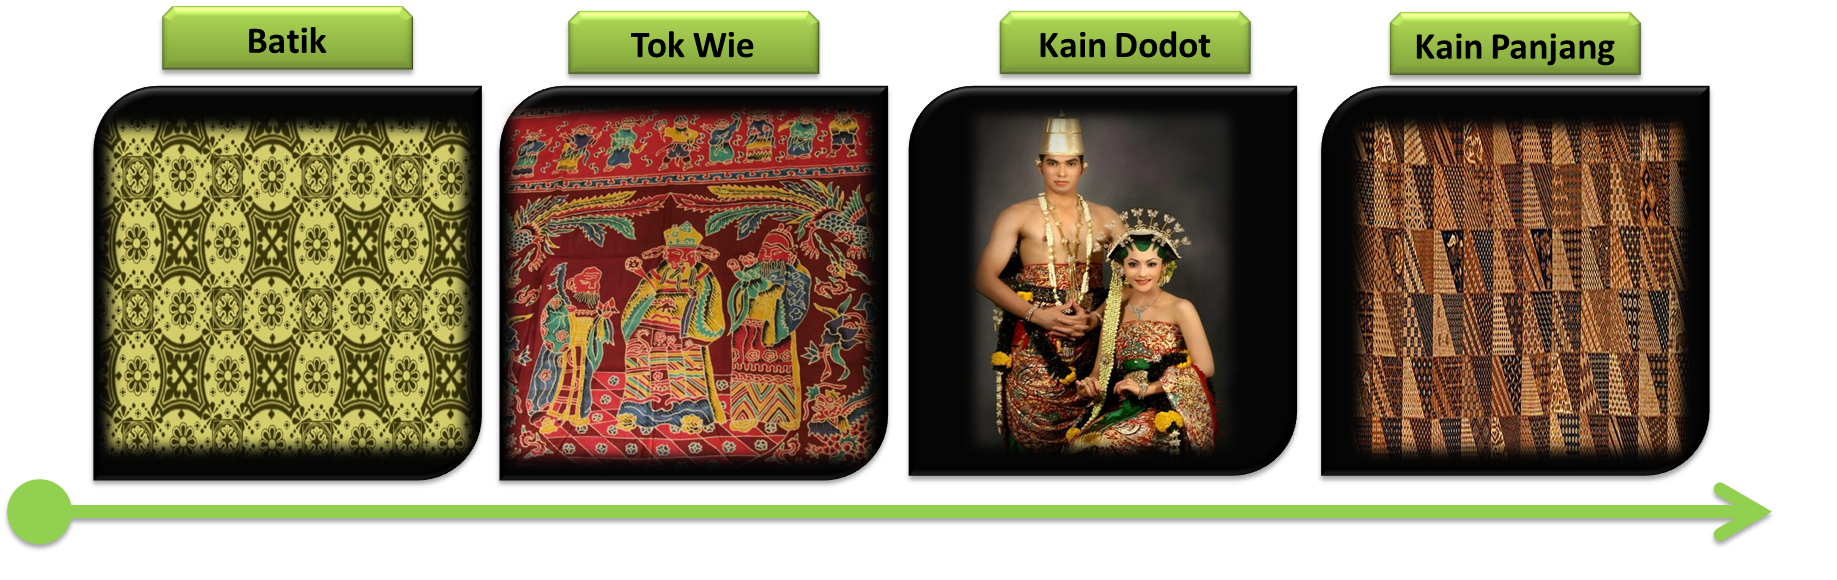
\includegraphics[width=10cm]{pics/kain_indonesia}
	\caption{Contoh kain dari berbagai daerah di indonesia}
	\label{fig:kain_indonesia}
\end{figure}
Salah satu kain tradisional Indonesia adalah batik. Batik merupakan kain bergambar yang memiliki gaya, warna dan tekstur dimana proses pembuatannya dilakukan secara manual maupun menggunakan mesin. Batik memiliki beberapa motif seperti motif kawung, motif parangkusumo, motif truntum, motif tambal, motif pamiluto, motif parang, motif liris maupun motif udan nitik seperti pada gambar \ref{fig:motif_batik}.

Tiap motif batik memiliki makna tersendiri berdasarkan daerah asal batik tersebut. Beberapa makna motif batik (sumber : http://batik-tulis.com/blog/batik-yogyakarta):
\begin{itemize}
	\item Motif ceplok dengan model grompol melambangkan harapan orang tua akan semua hal yang baik terkumpul, yaitu rejeki, kerukunan hidup, kebahagiaan, dan ketentraman untuk kedua mempelai dan keluarga pengantin.
	\item Motif kawung jogja melambangkan segala sesuatu yang bersifat murni, suci, dari putih kembali ke putih.
	\item Motif batik lereng dari yogyakarta melambangkan kesuburan, harapan untuk kemakmuran, tekad, untuk memiliki keberanian untuk melaksanakan apa yang penting bagi bangsa dan rakyat.
	\item Motif nitik dengan "motif cakar ayam biasa dikenakan pada acara perkawinan dengan tujuan agar pasangan yang menikah dapat mencari dengan halal sepandai ayam mencari makan dengan cakarnya".
	\item Motif parang menjadi "pedoman utama untuk menentukan derajat kebangsawanan seseorang dan menjadi pedoman yang termaktub dalam pranatan dalem asmanipun panganggo keprabon wonten kraton nagari ngayogjakarta hadiningrat pada tahun 1927".
\end{itemize} 
\begin{figure}[htp]
	\centering
	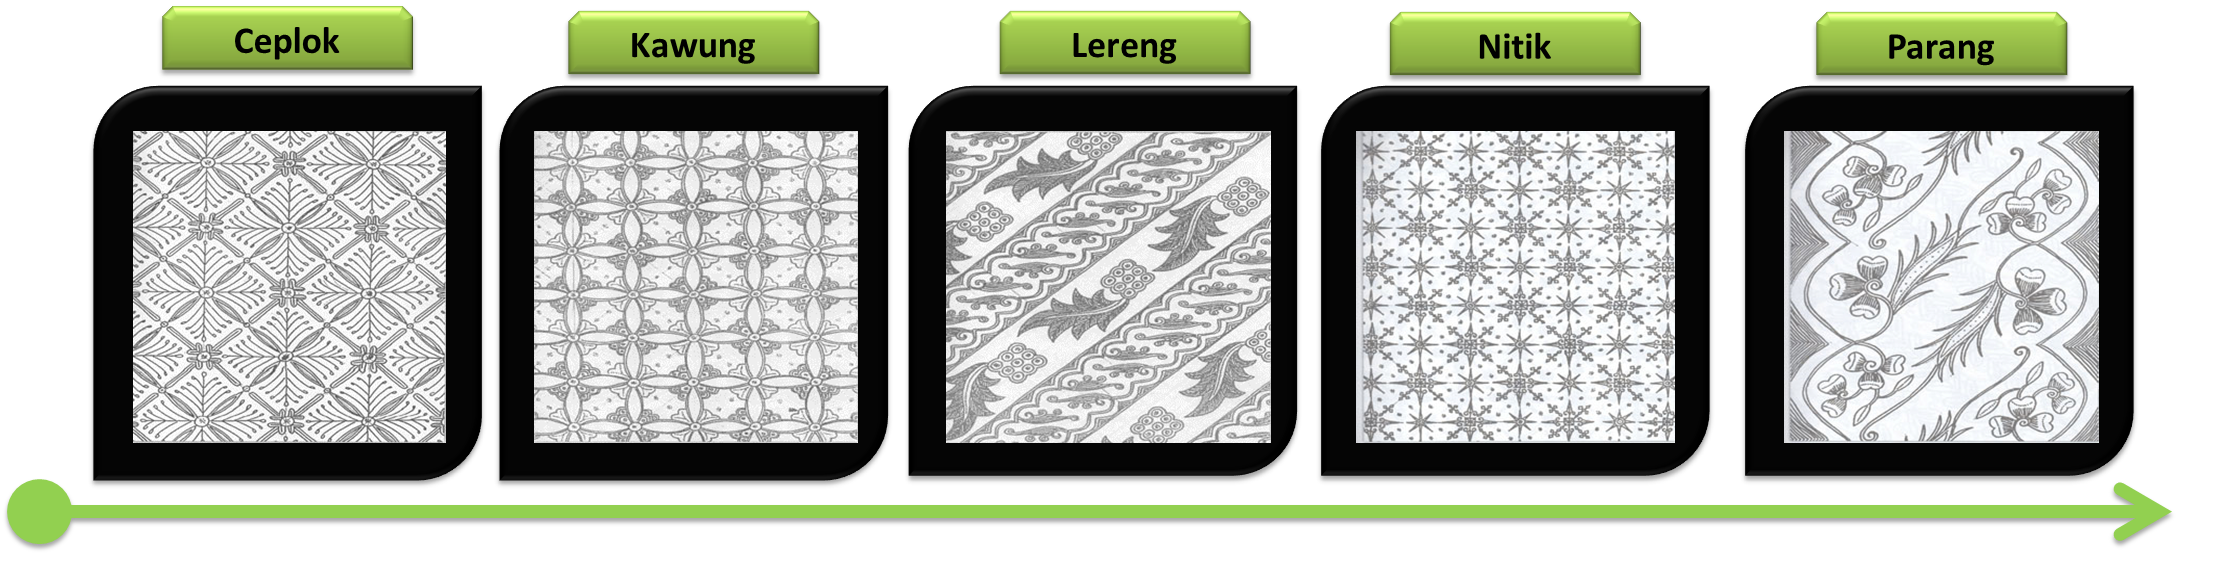
\includegraphics[width=15cm]{pics/motif_batik}
	\caption{Contoh motif batik indonesia}
	\label{fig:motif_batik}
\end{figure}
%-----------------------------------------------------------------------------%
\chapter{\babTiga}
%-----------------------------------------------------------------------------%
Metode yang digunakan dalam penelitian ini adalah metode kuantitatif dengan melakukan pengukuran akurasi dari pengujian data tes terhadap model yang terbentuk.


%-----------------------------------------------------------------------------%
\section{Teknik Pengumpulan Data}
%-----------------------------------------------------------------------------%
Sebelum melakukan penelitian, terlebih dahulu dilakukan proses pengumpulan data. Teknik yang digunakan untuk melakukan pengumpulan data adalah sebagai berikut:
\begin{enumerate}
	\item Studi literatur.\\
Sebelum mengumpulkan data, dilakukan proses studi literatur untuk menemukan jenis data yang tepat untuk melakukan penelitian ini.	
	\item Pengambilan data.\\
Proses pengambilan data dilakukan dengan mencari menggunakan teknologi internet dan search engine, misalnya dengan keyword “batik”, “batik Indonesia”, dll. Selain itu, dilakukan pengumpulan data secara langsung ke museum tekstil di Jakarta.
\end{enumerate}

%-----------------------------------------------------------------------------%
\section{Data}
Data yang digunakan dalam penelitian ini merupakan data primer yang diambil berdasarkan kata kunci di internet maupun pengambilan secara langsung seperti yang telah dijelaskan pada butir 3.1. Dalam penelitian ini, terdapat dua jenis data, yaitu data latih dan data uji. \\
Data latih yang diperlukan adalah kumpulan data batik yang memiliki variasi motif yang berasal dari berbagai daerah di Indonesia.

\section{Rancangan Penelitian}
Penelitian ini dilakukan di Fasilkom UI dengan metode penelitian kuantitatif yaitu dengan mengukur ketepatan prediksi asal daerah batik dari motif kain. Metode yang digunakan untuk membuat model prediksi motif kain adalah CNN dimana input akan dipecah menjadi ukuran yang lebih kecil dan diproses kedalam beberapa layer sehingga akan ditemukan fitur dari gambar yang kemudian menghasilkan model untuk melakukan deteksi asal daerah batik dari pola kain.\\
Alur kegiatan yang dilakukan dalam penelitian ini terdiri dari langkah, yaitu identifikasi masalah, studi literatur, pengumpulan data, Implementasi CNN, Implementasi Web Service, Implmentasi Web Service Client, Latih CNN, Uji CNN, Analisis hasil, Penarikan kesimpulan dan pembuatan laporan. Langkah-langkah tersebut dapat digambarkan dalam alur proses yang dapat dilihat pada gambar 3.1. Adapun target durasi waktu kerja dari langkah-langkah pada alur yang digambarkan pada tabel 3.2 dapat dilihat pada table project plan sebagai berikut.\\
\begin{table}
	\centering
	\caption{Project plan penelitian pengenalan batik dengan android}
	\label{tab:tab1}
	\begin{tabular}{| l|l|}
		\hline
		No & Deskripsi \\ 
		\hline
		1 & Identifikasi Masalah \\
		\hline
		2 & Studi Literatur \\
		\hline
		3 & Pengumpulan Data \\
		\hline
		4 & Implementasi CNN\\
		\hline
		5 & Implementasi Web Service\\				
		\hline
		6 & Implementasi Web Service Client\\
		\hline
		7 & Pelatihan CNN\\
		\hline
		8 & Pengujian CNN\\
		\hline
		9 & Analisis Hasil \\
		\hline
		10 & Penarikan Kesimpulan\\
		\hline
		11 & Pembuatan Laporan\\
		\hline
	\end{tabular}
\end{table}
\begin{table}
	\centering
	\caption{Timeline penelitian pengenalan batik dengan android}
	\label{tab:tab1}
	\begin{tabular}{|l|l|l|l|l|l|l|l|}
		\hline
		No & Deskripsi & Jul & Aug & Sep & Oct & Nov & Dec\\ 
		\hline
		1 & Identifikasi Masalah &x&&&&&\\
		\hline
		2 & Studi Literatur&x&&&&&\\
		\hline
		3 & Pengumpulan Data&&x&&&&\\
		\hline
		4 & Implementasi CNN&&x&x&x&&\\
		\hline
		5 & Implementasi Web Service&&x&x&x&&\\
		\hline
		6 & Implementasi Web Service Client&&x&x&x&&\\
		\hline
		7 & Pelatihan CNN&&x&x&x&&\\
		\hline
		8 & Pengujian CNN&&x&x&x&&\\
		\hline
		9 & Analisis Hasil&&&&&x&\\
		\hline
		10 & Penarikan Kesimpulan&&&&&x&\\
		\hline
		11 & Pembuatan Laporan&&&&&&x\\
		\hline
	\end{tabular}
\end{table}
Pengambilan data dilakukan pada bulan Maret 2016 pada museum tekstil jakarta, sedangkan pengambilan data via internet, dilakukan dari awal januari 2016 hingga saat ini.

\section{Pelatihan Model CNN}
Pelatihan motif kain dimulai dari input gambar yang sudah diberikan label secara manual berdasarkan kata kunci pencarian pada internet berdasarkan daerah asal batik dan data yang disediakan oleh museum tekstil. Gambar akan dijadikan input pada deeplearning4j dengan inisialisasi parameter:
\begin{itemize}
\item Seed
\item Iterations
\item Regularizations
\item L2
\item Learning rate
\item Weightinit
\item Optimization Algorithm
\item Updater
\end{itemize}

Setelah melakukan inisialisasi parameter, data gambar akan diproses kedalam layer dengan urutan sbb:
\begin{itemize}
	\item Layer 0 : Convolution Layer
	\item Layer 1 : Subsampling Layer  Max Pooling
	\item Layer 2 : Convolution Layer
	\item Layer 3 : Subsampling Layer  Max Pooling
	\item Layer 4 : Dense Layer
	\item Layer 5 : Output Layer
\end{itemize}

\begin{figure}[htp]
	\centering
	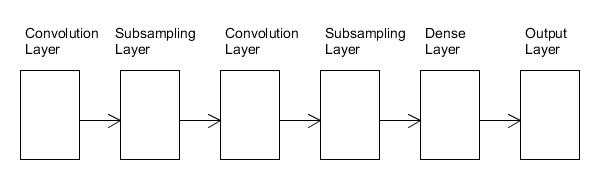
\includegraphics[width=8cm]{pics/arsitektur_cnn}
	\caption{Arsitektur CNN}
	\label{fig:arsitektur_cnn}
\end{figure}
Hasil dari output layer akan melakukan evaluasi terhadap data testing dan dilakukan pengukuran nilai . model hasil pembelajaran deeplearning4j akan disimpan dalam bentuk file biner sehingga bisa digunakan kembali untuk melakukan deteksi daerah asal kain batik.
\begin{figure}[htp]
	\centering
	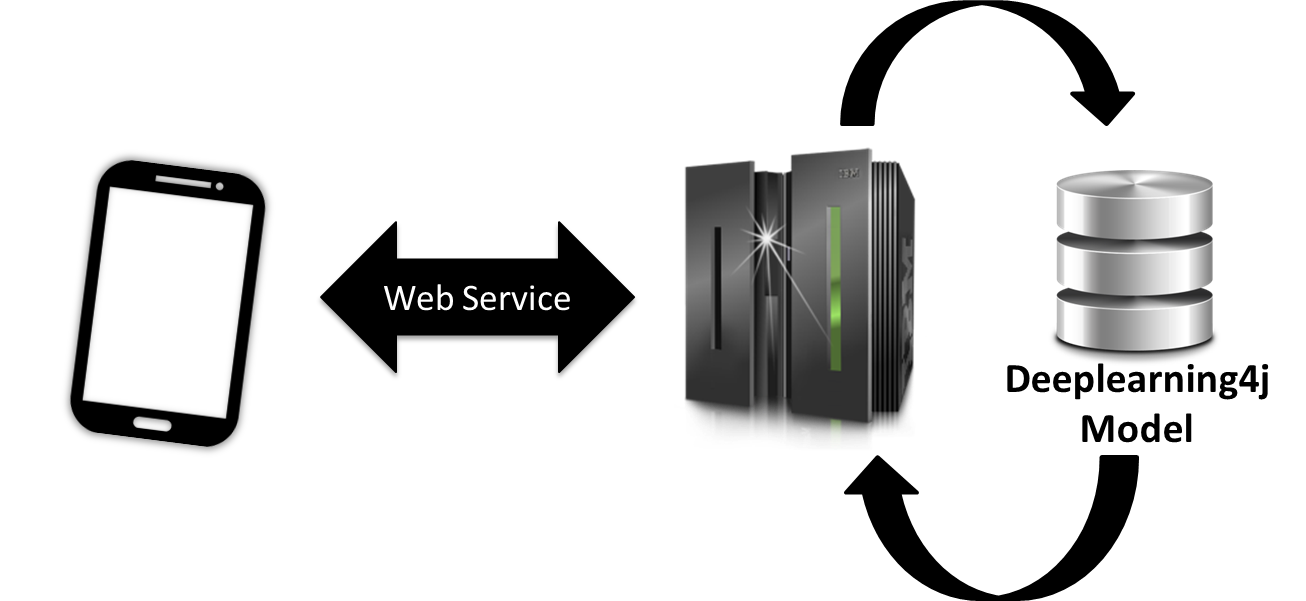
\includegraphics[width=8cm]{pics/komunikasi_cnn}
	\caption{Arsitektur Server untuk CNN}
	\label{fig:komunikasi_cnn}
\end{figure}
%%-----------------------------------------------------------------------------%
\chapter{\babEmpat}
%-----------------------------------------------------------------------------%
\todo{tambahkan kata-kata pengantar bab 1 disini}

%-----------------------------------------------------------------------------%
\section{thesis.tex}
%-----------------------------------------------------------------------------%
Berkas ini berisi seluruh berkas Latex yang dibaca, jadi bisa dikatakan sebagai 
berkas utama. Dari berkas ini kita dapat mengatur bab apa saja yang ingin 
kita tampilkan dalam dokumen.


%-----------------------------------------------------------------------------%
\section{laporan\_setting.tex}
%-----------------------------------------------------------------------------%
Berkas ini berguna untuk mempermudah pembuatan beberapa template standar. 
Anda diminta untuk menuliskan judul laporan, nama, npm, dan hal-hal lain yang 
dibutuhkan untuk pembuatan template. 


%-----------------------------------------------------------------------------%
\section{istilah.tex}
%-----------------------------------------------------------------------------%
Berkas istilah digunakan untuk mencatat istilah-istilah yang digunakan. 
Fungsinya hanya untuk memudahkan penulisan.
Pada beberapa kasus, ada kata-kata yang harus selalu muncul dengan tercetak 
miring atau tercetak tebal. 
Dengan menjadikan kata-kata tersebut sebagai sebuah perintah \latex~tentu akan 
mempercepat dan mempermudah pengerjaan laporan. 


%-----------------------------------------------------------------------------%
\section{hype.indonesia.tex}
%-----------------------------------------------------------------------------%
Berkas ini berisi cara pemenggalan beberapa kata dalam bahasa Indonesia. 
\latex~memiliki algoritma untuk memenggal kata-kata sendiri, namun untuk 
beberapa kasus algoritma ini memenggal dengan cara yang salah. 
Untuk memperbaiki pemenggalan yang salah inilah cara pemenggalan yang benar 
ditulis dalam berkas hype.indonesia.tex.


%-----------------------------------------------------------------------------%
\section{pustaka.tex}
%-----------------------------------------------------------------------------%
Berkas pustaka.tex berisi seluruh daftar referensi yang digunakan dalam 
laporan. 
Anda bisa membuat model daftar referensi lain dengan menggunakan bibtex.
Untuk mempelajari bibtex lebih lanjut, silahkan buka 
\url{http://www.bibtex.org/Format}. 
Untuk merujuk pada salah satu referensi yang ada, gunakan perintah \bslash 
cite, e.g. \bslash cite\{latex.intro\} yang akan akan memunculkan 
\cite{latex.intro}


%-----------------------------------------------------------------------------%
\section{bab[1 - 6].tex}
%-----------------------------------------------------------------------------%
Berkas ini berisi isi laporan yang Anda tulis. 
Setiap nama berkas e.g. bab1.tex merepresentasikan bab dimana tulisan tersebut 
akan muncul. 
Sebagai contoh, kode dimana tulisan ini dibaut berada dalam berkas dengan nama 
bab4.tex. 
Ada enam buah berkas yang telah disiapkan untuk mengakomodir enam bab dari 
laporan Anda, diluar bab kesimpulan dan saran. 
Jika Anda tidak membutuhkan sebanyak itu, silahkan hapus kode dalam berkas 
thesis.tex yang memasukan berkas \latex~yang tidak dibutuhkan;  contohnya 
perintah \bslash include\{bab6.tex\} merupakan kode untuk memasukan berkas 
bab6.tex kedalam laporan.


%%-----------------------------------------------------------------------------%
\chapter{\babLima}
%-----------------------------------------------------------------------------%
\todo{Tambahkan kata-kata pengantar bab 5 disini.}


%-----------------------------------------------------------------------------%
\section{Mengubah Tampilan Teks}
%-----------------------------------------------------------------------------%
Beberapa perintah yang dapat digunakan untuk mengubah tampilan adalah: 
\begin{itemize}
	\item \bslash f \\
		Merupakan alias untuk perintah \bslash textit, contoh 
		\f{contoh hasil tulisan}.
	\item \bslash bi \\
		\bi{Contoh hasil tulisan}.
	\item \bslash bo \\
		\bo{Contoh hasil tulisan}.
	\item \bslash m \\
		\m{Contoh hasil tulisan}.
	\item \bslash mc \\
		\mc{Contoh hasil tulisan}.
	\item \bslash code \\ 
		\code{Contoh hasil tulisan}.
\end{itemize}


%-----------------------------------------------------------------------------%
\section{Memberikan Catatan}
%-----------------------------------------------------------------------------%
Ada dua perintah untuk memberikan catatan penulisan dalam dokumen yang Anda 
kerjakan, yaitu: 
\begin{itemize}
	\item \bslash todo \\
		Contoh: \\ \todo{Contoh bentuk todo.}
	\item \bslash todoCite \\ 
		Contoh: \todoCite
\end{itemize}


%-----------------------------------------------------------------------------%
\section{Menambah Isi Daftar Isi}
%-----------------------------------------------------------------------------%
Terkadang ada kebutuhan untuk memasukan kata-kata tertentu kedalam Daftar Isi. 
Perintah \bslash addChapter dapat digunakan untuk judul bab dalam Daftar isi. 
Contohnya dapat dilihat pada berkas thesis.tex.


%-----------------------------------------------------------------------------%
\section{Memasukan PDF}
%-----------------------------------------------------------------------------%
Untuk memasukan PDF dapat menggunakan perintah \bslash inpdf yang menerima satu 
buah argumen. Argumen ini berisi nama berkas yang akan digabungkan dalam 
laporan. PDF yang dimasukan degnan cara ini akan memiliki header dan footer 
seperti pada halaman lainnya. 

\inpdf{include}

Cara lain untuk memasukan PDF adalah dengan menggunakan perintah \bslash putpdf 
dengan satu argumen yang berisi nama berkas pdf. Berbeda dengan perintah 
sebelumnya, PDF yang dimasukan dengan cara ini tidak akan memiliki footer atau 
header seperti pada halaman lainnya. 

\putpdf{include}


%-----------------------------------------------------------------------------%
\section{Membuat Perintah Baru}
%-----------------------------------------------------------------------------%
Ada dua perintah yang dapat digunakan untuk membuat perintah baru, yaitu: 
\begin{itemize}
	\item \bslash Var \\
		Digunakan untuk membuat perintah baru, namun setiap kata yang diberikan
		akan diproses dahulu menjadi huruf kapital. 
		Contoh jika perintahnya adalah \bslash Var\{adalah\} makan ketika 
		perintah \bslash Var dipanggil, yang akan muncul adalah ADALAH. 
	\item \bslash var \\
		Digunakan untuk membuat perintah atau baru. 
\end{itemize}


%%-----------------------------------------------------------------------------%
\chapter{\babEnam}
%-----------------------------------------------------------------------------%
\todo{tambahkan kata-kata pengantar bab 6 disini}


%%---------------------------------------------------------------
\chapter{\kesimpulan}
%---------------------------------------------------------------
\todo{Tambahkan kesimpulan dan saran terkait dengan perkerjaan 
	yang dilakukan.}


%---------------------------------------------------------------
\section{Kesimpulan}
%---------------------------------------------------------------


%---------------------------------------------------------------
\section{Saran}
%---------------------------------------------------------------


%
% Daftar Pustaka
%
% Daftar Pustaka 
% 

% 
% Tambahkan pustaka yang digunakan setelah perintah berikut. 
% 
\begin{thebibliography}{4}

\bibitem Yizhang Xia, Bailing Zhang, Frans Coenen. Face Occlusion Detection Based on Multi-task Convolution Neural Network. 2015 12th International Conference on Fuzzy Systems and Knowledge Discovery (FSKD)

\bibitem Earnest Paul Ijjina, C Krishna Mohan. Human Action Recognition based on Motion Capture Information using Fuzzy Convolution Neural Networks. 

\bibitem Hsien-I Lin†, Ming-Hsiang Hsu, and Wei-Kai Chen. Human Hand Gesture Recognition Using a Convolution Neural Network. 2014 IEEE International Conference on Automation Science and Engineering (CASE) Taipei, Taiwan, August 18-22, 2014

\bibitem Yizhang Xia, Bailing Zhang, Frans Coenen. Face Occlusion Detection Based on Multi-task Convolution Neural Network. 2015 12th International Conference on Fuzzy Systems and Knowledge Discovery (FSKD)

\bibitem Earnest Paul Ijjina, C Krishna Mohan. Human Action Recognition based on Motion Capture Information using Fuzzy Convolution Neural Networks. 

\bibitem Hsien-I Lin†, Ming-Hsiang Hsu, and Wei-Kai Chen. Human Hand Gesture Recognition Using a Convolution Neural Network. 2014 IEEE International Conference on Automation Science and Engineering (CASE) Taipei, Taiwan, August 18-22, 2014

\bibitem Nanik Suciati, Agri Kridanto, Mohammad Farid Naufal, Muhammad Machmud \& Ardian Yusuf Wicaksono. Fast Discrete Curvelet Transform And HSV Color Features For Batik Image Classification. 2015 International Conference on Information, Communication Technology and System (ICTS)

\bibitem Xinyan Yu1, Guohao Lyu, Siwei Luo, Junbo Liu. A Convolution Neural Network Based Variational Restoration Model

\bibitem Nanik Suciati, Agri Kridanto, Mohammad Farid Naufal, Muhammad Machmud \& Ardian Yusuf Wicaksono. Fast Discrete Curvelet Transform And HSV Color Features For Batik Image Classification. 2015 International Conference on Information, Communication Technology and System (ICTS)

\bibitem L. M. Rasdi Rere, Mohamad Ivan Fanany, Aniati Murni Arymurthy.Metaheuristic Algorithms for Convolution Neural Network. Hindawi Publishing Corporation Computational Intelligence and Neuroscience

\bibitem yejun Tang, Liangrui Peng, Qian Xu, Yanwei Wang dan Akio Furuhata. CNN based Transfer Learning for Historical Chinese Character Recognition. 2016 12th IAPR Workshop on Document Analysis Systems

\end{thebibliography}



%
% Lampiran 
%
%\begin{appendix}
%	%
% @author  Andreas Febrian
% @version 1.00 
% 
% Hanya sebuah pembatas bertuliskan LAMPIRAN ditengah halaman. 
% 

\begin{titlepage}
	\centering 
	\vspace*{6cm}
	\noindent \Huge{LAMPIRAN}
	\addChapter{LAMPIRAN}
\end{titlepage}
%	\setcounter{page}{2}
%	%-----------------------------------------------------------------------------%
\addChapter{Lampiran 1}
\chapter*{Lampiran 1}
%-----------------------------------------------------------------------------%
%\end{appendix}

\end{document}